\chapter{Marco teório: arquitectura de procesadores}
\label{ch:theory}

En líneas generales un procesador es un sistema que permite, por un lado
ingresar instrucciones y datos obteniendo en consecuencia los resultados de
operar lo indicado en las instrucciones sobre los datos. No es necesario para
tal fin, definir ninguna tecnología que soporte este comportamiento; se trata
más bien de un desarrollo teórico. Dicho desarrollo implica distinguir las
distintas partes que lo componen. En un primera aproximación, en un sistema de
procesamiento podemos distinguir cuatro componentes:

\begin{itemize}
  \item Datos de entrada
  \item Instrucciones
  \item Unidad de procesamiento
  \item Datos de salida
\end{itemize}

\begin{figure}
  \centering
  % Graphic for TeX using PGF
% Title: /home/lnatale/Documents/xfire/digital/xfire_core/docs/thesis/tesis/figures/C02-sistema_de_procesamiento.dia
% Creator: Dia v0.97.3
% CreationDate: Thu May 26 20:46:38 2016
% For: lnatale
% \usepackage{tikz}
% The following commands are not supported in PSTricks at present
% We define them conditionally, so when they are implemented,
% this pgf file will use them.
\ifx\du\undefined
  \newlength{\du}
\fi
\setlength{\du}{15\unitlength}
\begin{tikzpicture}
\pgftransformxscale{0.750000}
\pgftransformyscale{-0.750000}
\definecolor{dialinecolor}{rgb}{0.000000, 0.000000, 0.000000}
\pgfsetstrokecolor{dialinecolor}
\definecolor{dialinecolor}{rgb}{1.000000, 1.000000, 1.000000}
\pgfsetfillcolor{dialinecolor}
\definecolor{dialinecolor}{rgb}{1.000000, 1.000000, 1.000000}
\pgfsetfillcolor{dialinecolor}
\fill (4.707500\du,-42.000000\du)--(4.707500\du,-36.100000\du)--(8.672500\du,-36.100000\du)--(8.672500\du,-42.000000\du)--cycle;
\pgfsetlinewidth{0.100000\du}
\pgfsetdash{}{0pt}
\pgfsetdash{}{0pt}
\pgfsetmiterjoin
\definecolor{dialinecolor}{rgb}{0.000000, 0.000000, 0.000000}
\pgfsetstrokecolor{dialinecolor}
\draw (4.707500\du,-42.000000\du)--(4.707500\du,-36.100000\du)--(8.672500\du,-36.100000\du)--(8.672500\du,-42.000000\du)--cycle;
% setfont left to latex
\definecolor{dialinecolor}{rgb}{0.000000, 0.000000, 0.000000}
\pgfsetstrokecolor{dialinecolor}
\node at (6.690000\du,-39.255000\du){Datos de};
% setfont left to latex
\definecolor{dialinecolor}{rgb}{0.000000, 0.000000, 0.000000}
\pgfsetstrokecolor{dialinecolor}
\node at (6.690000\du,-38.455000\du){entrada};
\definecolor{dialinecolor}{rgb}{1.000000, 1.000000, 1.000000}
\pgfsetfillcolor{dialinecolor}
\fill (21.000000\du,-42.000000\du)--(21.000000\du,-36.100000\du)--(24.965000\du,-36.100000\du)--(24.965000\du,-42.000000\du)--cycle;
\pgfsetlinewidth{0.100000\du}
\pgfsetdash{}{0pt}
\pgfsetdash{}{0pt}
\pgfsetmiterjoin
\definecolor{dialinecolor}{rgb}{0.000000, 0.000000, 0.000000}
\pgfsetstrokecolor{dialinecolor}
\draw (21.000000\du,-42.000000\du)--(21.000000\du,-36.100000\du)--(24.965000\du,-36.100000\du)--(24.965000\du,-42.000000\du)--cycle;
% setfont left to latex
\definecolor{dialinecolor}{rgb}{0.000000, 0.000000, 0.000000}
\pgfsetstrokecolor{dialinecolor}
\node at (22.982500\du,-39.255000\du){Datos de};
% setfont left to latex
\definecolor{dialinecolor}{rgb}{0.000000, 0.000000, 0.000000}
\pgfsetstrokecolor{dialinecolor}
\node at (22.982500\du,-38.455000\du){salida};
% setfont left to latex
\definecolor{dialinecolor}{rgb}{0.000000, 0.000000, 0.000000}
\pgfsetstrokecolor{dialinecolor}
\node[anchor=west] at (22.982500\du,-39.050000\du){};
\definecolor{dialinecolor}{rgb}{1.000000, 1.000000, 1.000000}
\pgfsetfillcolor{dialinecolor}
\fill (12.000000\du,-42.000000\du)--(12.000000\du,-36.100000\du)--(18.000000\du,-36.100000\du)--(18.000000\du,-42.000000\du)--cycle;
\pgfsetlinewidth{0.100000\du}
\pgfsetdash{}{0pt}
\pgfsetdash{}{0pt}
\pgfsetmiterjoin
\definecolor{dialinecolor}{rgb}{0.000000, 0.000000, 0.000000}
\pgfsetstrokecolor{dialinecolor}
\draw (12.000000\du,-42.000000\du)--(12.000000\du,-36.100000\du)--(18.000000\du,-36.100000\du)--(18.000000\du,-42.000000\du)--cycle;
% setfont left to latex
\definecolor{dialinecolor}{rgb}{0.000000, 0.000000, 0.000000}
\pgfsetstrokecolor{dialinecolor}
\node at (15.000000\du,-39.255000\du){Unidad de};
% setfont left to latex
\definecolor{dialinecolor}{rgb}{0.000000, 0.000000, 0.000000}
\pgfsetstrokecolor{dialinecolor}
\node at (15.000000\du,-38.455000\du){procesamiento};
\definecolor{dialinecolor}{rgb}{1.000000, 1.000000, 1.000000}
\pgfsetfillcolor{dialinecolor}
\fill (12.000000\du,-48.000000\du)--(12.000000\du,-44.350000\du)--(18.000000\du,-44.350000\du)--(18.000000\du,-48.000000\du)--cycle;
\pgfsetlinewidth{0.100000\du}
\pgfsetdash{}{0pt}
\pgfsetdash{}{0pt}
\pgfsetmiterjoin
\definecolor{dialinecolor}{rgb}{0.000000, 0.000000, 0.000000}
\pgfsetstrokecolor{dialinecolor}
\draw (12.000000\du,-48.000000\du)--(12.000000\du,-44.350000\du)--(18.000000\du,-44.350000\du)--(18.000000\du,-48.000000\du)--cycle;
% setfont left to latex
\definecolor{dialinecolor}{rgb}{0.000000, 0.000000, 0.000000}
\pgfsetstrokecolor{dialinecolor}
\node at (15.000000\du,-45.980000\du){Instrucciones};
\pgfsetlinewidth{0.100000\du}
\pgfsetdash{}{0pt}
\pgfsetdash{}{0pt}
\pgfsetbuttcap
{
\definecolor{dialinecolor}{rgb}{0.000000, 0.000000, 0.000000}
\pgfsetfillcolor{dialinecolor}
% was here!!!
\pgfsetarrowsend{latex}
\definecolor{dialinecolor}{rgb}{0.000000, 0.000000, 0.000000}
\pgfsetstrokecolor{dialinecolor}
\draw (8.720837\du,-39.050000\du)--(11.950193\du,-39.050000\du);
}
\pgfsetlinewidth{0.100000\du}
\pgfsetdash{}{0pt}
\pgfsetdash{}{0pt}
\pgfsetbuttcap
{
\definecolor{dialinecolor}{rgb}{0.000000, 0.000000, 0.000000}
\pgfsetfillcolor{dialinecolor}
% was here!!!
\pgfsetarrowsend{latex}
\definecolor{dialinecolor}{rgb}{0.000000, 0.000000, 0.000000}
\pgfsetstrokecolor{dialinecolor}
\draw (15.000000\du,-44.301556\du)--(15.000000\du,-42.049771\du);
}
\pgfsetlinewidth{0.100000\du}
\pgfsetdash{}{0pt}
\pgfsetdash{}{0pt}
\pgfsetbuttcap
{
\definecolor{dialinecolor}{rgb}{0.000000, 0.000000, 0.000000}
\pgfsetfillcolor{dialinecolor}
% was here!!!
\pgfsetarrowsend{latex}
\definecolor{dialinecolor}{rgb}{0.000000, 0.000000, 0.000000}
\pgfsetstrokecolor{dialinecolor}
\draw (18.050441\du,-39.050000\du)--(20.950821\du,-39.050000\du);
}
\end{tikzpicture}

  \captionsetup{justification=centering}
  \caption{Esquema simplificado de un ``sistema de procesamiento''}
  \label{fig:C02-sistema_de_procesamiento}
\end{figure}

Estos componentes se relacionan de la forma mostrada en la figura
\ref{fig:C02-sistema_de_procesamiento}. Debe notarse que los datos de entrada y
las instrucciones ingresan a la unidad de procesamiento, la cual genera datos de
salida como resultado de operar las instrucciones sobre los datos de entrada.\\
Los datos de entrada representan el dominio sobre el cual puede operar la unidad
de procesamiento. Para definir un sistema de procesamiento debemos especificar,
entonces, cuál es el dominio que puede manejar. Dicha definición deberá
especificar el formato y cantidad de datos que acepta la unidad de
procesamiento, así como los mecanismos para ingresarlos al sistema.\\
Las instrucciones definirán las operaciones que la unidad de procesamiento
puede realizar sobre los datos de entrada. Por lo tanto, para definir un sistema
de procesamiento, debemos definir qué operaciones será capaz de realizar sobre
el dominio de entrada del mismo. A su vez, se debe definir la salida esperada de
las instrucciones; es por eso que al definir las instrucciones estamos
definiendo intrínsecamente el dominio de salida del sistema. Es importante notar
que la información sobre las instrucciones también representa una entrada para
el sistema, es por eso que, como en el caso de los datos de entrada, se deberá
especificar formato y cantidad que acepta la unidad de procesamiento, así como
los mecanismos para ingresarlas.\\
Los datos de salida representan el dominio sobre el cuál las instrucciones
vuelcan el resultado de las operaciones realizadas sobre los datos de entrada.
El dominio de salida, como fue notado antes, queda definido al definir las
instrucciones, pero debe definirse el formato y cantidad de los mismos, así como
los mecanismos necesarios para extraerlos del sistema.\\
En este contexto la unidad de procesamiento es la encargada de recibir las
instrucciones y datos, ejecutar las operaciones para finalmente presentar los
resultados.\\
Un microprocesadores es ---en efecto--- una implementación de un sistema de
procesamiento. El sustento físico de dicha implementación es la
microelectrónica. En las siguientes secciones de este capítulo, se repasará el
marco histórico en el que surgen los microprocesadores y las arquitecturas
asociadas.

\section{Perspectiva histórica}
\label{sec:theory-history}

Desde épocas remotas, el hombre se ha destacado en el mundo animal por su
capacidad de modificar su entorno para resolver problemas recurrentes. Es esta
capacidad la fortaleza de la especie en la naturaleza. La película ``2001:
Odisea del esapcio''\footnote{``2001: Odisea en el espacio'': es un film del año
1968 dirigida por Stanley Kubrick basada en la novela de Arthur C. Clarke.}
narra, desde un enfoque particular, parte de la evolución del ser humano, o al
menos la interpretación de los autores sobre la misma. En la misma, ubicándose
temporalmente varios millones de años atrás, un clan de cavernícolas prehumanos
intentan sobrevivir en condiciones extremas. Comen los pocos hierbajos que
pueden encontrar en el desolado paisaje, hierbajos que para colmo han de
compartir con una manada de tapires que habita la misma zona. La única fuente de
agua del clan —un simple charco— les es arrebatada por un clan rival. Por si
fuera poco, este desdichado clan vive permanentemente amenazado por un leopardo
que domina la región y que de vez en cuando caza a alguno de sus miembros. En
resúmen: este grupo de homínidos padece hambre, frío y miedo, y parecen
condenados a una segura extinción. En ese contexto, y por motivos que no vienen
al caso, aparece uno de los cavernícolas contemplando el esqueleto de un animal.
Parece reflexionar sobre lo que tiene delante, como si estuviese viéndolo desde
una nueva perspectiva. Hay algo nuevo en aquellos huesos. Algo que hasta
entonces ni él ni ninguno de sus congéneres habían visto. Los huesos que hay
tirados por el suelo pueden ser usados. El cavernícola toma el más robusto de
los huesos y empieza a golpear el esqueleto; primero con precaución, más tarde
con fuerza, hasta que termina consumido por un frenesí violento. Este
cavernícola acaba de descubrir el primer arma —la primera herramienta— de la
historia. O dicho de otro modo, acaba de aparecer el primer ser humano sobre la
faz de la tierra. Gracias al uso del hueso —o de herramientas similares como
palos o piedras— el clan que estaba a punto de extinguirse descubre que puede
cazar a los tapires con los que convive y comérselos. Así que sus problemas de
hambre han terminado. También gracias a sus armas pueden atacar al clan rival y
recuperar el charco de agua, lo que soluciona también sus problemas de sed. Y
deducimos que serán capaces incluso de defenderse del peligroso leopardo. Los
miembros del clan ya no son prehumanos indefensos; ahora son humanos armados.\\
Esta cita cinematográfica pretende graficar la diferenciación del ser humano en
la cadena alimenticia. Gracias al poder de la observación y el razonamiento
hemos sido capaces de modificar nuestro entorno para asegurar la supervivencia
de la especie en un mundo en el que la misma se encontraba en clara desventaja.
En este contexto, el ser humano ha sido capaz de generar un desarollo
tecnológico, que hoy en día es vertiginoso.\\

\subsection{La ``Máquina de Turing''}
\label{subsec:theory-history-turing}

Alan Mathison Turing\footnote{Alan Mathison Turing (23 June 1912 – 7 June 1954):
típicamente considerado el padre de las ciencias de la computación y de la
inteligencia artificial, fue un biólogo, matemático, lógico, científico de la
computación y de la criptografía inglés que formalizó los conceptos de algoritmo
y computación mediante la ``Máquina de Turing'', que es un modelo de una
computadora de propósito general} es considerado el padre de la computación y
la inteligencia artificial. Sus trabajos en el campo de la computación se
remontan al año 1936 cuando publica un \emph{paper} llamado ``On computable
Numbers, with an Application to the Entscheidungsproblem''. En este contexto,
Turing inventó la llamada Máquina de Turing; esta máquina se trata de un modelo
abstracto que manipula símobolos ingresados a través de un medio infinito, de
acuerdo a una tabla de reglas, o para ser más exactos, es la definición del
modelo matemático de una máquina capaz de hacer dicho trabajo. A pesar de la
simplicidad del modelo planteado por Turing, dado cualquier algoritmo
computable, una Máquina de Turing que lo resuelva puede ser construída. Con éste
modelo, reformuló los resultados hallados por Kurt Gödel en 1931 sobre los
límites de prueba y computabilidad, reemplazando el lenguaje formal planteado
por Gödel, por su modelo de máquina. Turing demostró que cualquier problema que
pudiera ser representado por un algoritmo, podía ser resuelto por una Máquina de
Turing, a su vez probando que el ``problema de decisión'' (entscheidungsproblem)
no tenía solución, al probar que el ``Halting Problem'' (Problema de Parada)
para las Máquinas de Turing es indeterminado según el problema de decisión. En
otras palabras, para un problema de este tipo, está indeterminado el hecho de
que la máquina termine de computar. Es así que la Máquina de Turing fué capaz de
demostrar las limitaciones del poder de cómputo. El modelo de acceso de datos e
instrucciones era secuencial, lo cuál es minimalista, pero no apto para
implementaciones prácticas. La teoría de autómatas es la rama de la ciencia que
hoy se ocupa de estudiar estos modelos matemáticos de computabilidad. Se
establece así la propiedad de que un sistema arbitrario de instrucciones sea
``Turing-Completo''.

\subsection{La revolución digital}
\label{subsec:theory-history-digital_revolution}

La revolución digital es considerada la tercera revolución industrial, dando
orígen a la llamada ``Era de la Información''. Sus comienzos se remontan a fines
de los años 50. La adopción y proliferación de las computadoras digitales y el
mantenimiento de registros digitales de información son las características que
la definen. De manera implícita, esta revolución está relacionada con los
cambios radicales provocados por la computación y las tecnologías de
telecomunicaciones. En el corazón de este proceso encontramos dos componentes
tecnológicas. Por un lado está la teoría, que puede remontarse a los primeros
análisis matemáticos de la lógica, como el álgebra de Boole introducida por
primera vez en un pequeño folleto publicado en 1847 bajo el nombre \emph{The
Mathematical Analisis of Logic} y la posterior publicación del libro \emph{An
Investigation of the Laws of Thought on Which are Founded the Mathematical
Theories of Logic and Probabilities}, publicado en 1854. En estas publicaciónes
George Boole\footnote{George Boole (2 de Noviembre de 1815 - 8 de Diciembre de
1864): Matemático, docente, filósofo y lógico Ingles. Trabajó en los campos de
las ecuaciones diferenciales y el álgebra lógica. Su obra ``The Laws of
Thaught'' (Las Leyes del Pensamiento) de 1854 describen lo que hoy conocemos
como Álgebra de Boole, piedra fundamental de la ``Era de la Información''.}
pretendió utilizar técnicas algebraicas para tratar expresiones de la lógica
proposicional. En la actualidad, el álgebra de Boole se aplica de forma
generalizada en el ámbito del diseño electrónico. Claude Shannon\footnote{Claude
Elwood Shannon (30 de Abril de 1916 - 24 de Febrero de 2001): Matemático,
ingeniero eléctrico y cryptografista nacido en Estados Unidos de América, es
conocido como el padre de la teoría de la información. Con un \emph{paper}
publicado en 1948, describió lo que hoy conocemos como teoría de la información.
Pero previamente, en 1937, también trabajó en lo que hoy conocemos como la
teoría del diseño de circuitos digitales, al realizar su tesis de maestría
aplicando las leyes del Álgebra de Boole a circuitos eléctricos, demostrando que
podía construirse cualquier función lógica y numérica.} fué el primero en
aplicarla en el diseño de circuitos de conmutación eléctrica biestables, en
1948. Por el otro lado, se encuentra la revolución del silicio y la producción
en masa y uso generalizado de circuitos lógicos digitales que permitieron el
desarrollo en gran escala de circuitos electrónicos que implementan funciones
lógicas basados en los desarrollos de Boole. Aproximadamente cien años pasaron
desde que Boole publicó su teoría, hasta que la tecnología encontró el camino
para implementar esos conocimientos de forma práctica y útil. La invención del
transistor data del año 1947. En la figura \ref{fig:C02-primer_transistor} se
muestra una imágen de una réplica de este primer transistor de la historia. Este
invento fué el que permitió la creación de equipos digitales avanzados. En el
contexto de la lógica digital, los transistores son utilizados como llaves de
conmutación que permiten o no el paso de una señal eléctrica al ser excitados
por otra señal. Previo a los transistores, la lógica era implementada con
componentes electromecánicos y válvulas termoiónicas de vacío; tecnologías que
por su naturaleza eran de dimensiones y consumos energéticos elevados y poco
fiables. Para poner esta problemática en perspectiva, comparamos la primera
computadora de propósito general electrónica, llamada
ENIAC\footnote{``Electronic Numerical Integrator and Computer'' (Integrador
numérico y computadora electróica): Considerada la primera computadora
electrónica de propósito general. Era ``Touring-complete'', digital y podía
resolver una gran cantidad de problemas numéricos al ser reprogramable.}
implementada con 18000 válvulas, con un consumo de $160\,\mathrm{KW}$, capaz de
realizar $5000\,\mathrm{sumas/s}$, $385\,\mathrm{multiplicaciones/s}$, con 5
millones de soldaduras y un peso de $30\,\mathrm{Ton}$, contra un procesador
Intel Core I7 de última generación que permite $177000\,\mathrm{MIPS}$ con un
consumo de aproximadamente $100\,\mathrm{W}$, es decir, 35 millones de veces más
rápido. Para hacer la misma cantidad de sumas por segundo se requerirían
$5\,\mathrm{GW}$ con la ENIAC; considerar que la capacidad actual instalada en
argentina es de $30\,\mathrm{GW}$.
\begin{figure}
  \centering
  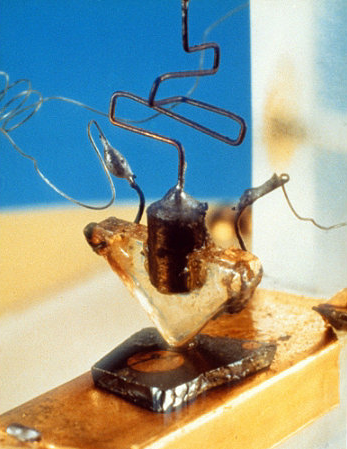
\includegraphics[scale=0.5]{./figures/C02-primer_transistor}
  \captionsetup{justification=centering}
  \caption{Primer transistor desarrollado por John Bardeen y Walter 
    Brattain bajo la dirección de William Shockley en los Laboratorios Bell de 
    AT\&T en el año 1947}.
  \label{fig:C02-primer_transistor}
\end{figure}

\subsection{Silicio, dispositivos semiconductores y transistores}
\label{subsec:theory-history-semiconductors}

Los semiconductores son materiales, que como bien indica su nombre, no son del
todo conductores. En ellos, la capacidad de conducir una corriente eléctrica
puede ser manipulada de diversas maneras. En 1931 Wolfgang Pauli ---quien en 
1945 fue premiado con el Nobel de Física--- enunció: ``Uno no debería trabajar 
en semiconductores, eso es un lío deleznable, quién sabe si realmente existen''.
Nada más alejado de la realidad que hoy nos rodea. Los materiales
semiconductores permitieron la creación de los transistores y posteriormente los
circuitos integrados, dispositivos que iniciaron la revolución digital. Los
primeros dispositivos fueron fabricados sobre germanio y arsenurio de galio.
Incluso, el primer circuito integrado, fue realizado en germanio. Pero fue el 
silicio el material que realmente revolucionó la industria, por su alta
disponibilidad en la naturaleza y relativa fácil manipulación para la
fabricación de dispositivos semiconductores en circuitos integrados. Puede
afirmarse que el silicio es uno de los materiales mejor conocidos por el ser
humano. Hace más de 50 años que se lo estudia en detalle para mejorar la
tecnología, logrando importantes avances. También puede afirmarse que los
transistores hoy en día conforman el bien más abundante en el mundo. Una
comparativa del año 2012 muestra que durante año se produjeron en el órden de
$10^{17}$ granos de arroz en la tierra, mientras que en el mismo período en se
produjeron en el órden de $10^{19}$ transistores, según declaraciones de la
\emph{Semiconductor Industry Asociation} de los Estados Unidos de América. La
clave de semejante número en la producción son los circuitos integrados.

\subsection{Circuitos integrados y tencología CMOS}
\label{subsec:theory-history-ic}

En la figura \ref{fig:C02-primer_circuito_integrado} puede verse el primer
circuito integrado de la historia. Medía aproximadamente media pulgada de ancho
e implementaba dos transistores montados en una barra de germanio. Nace así el
concepto del \emph{chip} o \emph{microchip}: en inglés, \emph{chip} significa
``corte o fracción pequeño de un material duro'' directamente relacionado con la
técnica de fabricación de circuitos integrados donde, a grandes rasgos, una
barra cilíndrica de cristal de silicio puro, es cortada en muy delgadas láminas
en forma de discos, sobre las cuales se ``imprimen'' los circuitos integrados,
repitiendo el mismo patrón múltiples veces en un mismo disco para finalmente
cortar ese disco en diminutos fragmentos que contienen el diseño. La evolución
de las técnicas de fabricación permitieron integrar en un mismo \emph{chip} de
silicio más de un dispositivo, permitiendo implementar circuitos relativamente
complejos en una pequeña área de silicio, disminuyendo así los riesgos de fallas
por interconexión entre dispositivos. A su vez, las técnicas de fabricación
evolucionaron permitiendo escalar el tamaño de los dispositivos fabricados
incrementando la cuenta de dispositivos integrados por unidad de área. Como
consecuencia buscada de disminuir el tamaño de los dispositivos, se logró
aumentar la velocidad máxima de conmutación que los mismos pueden lograr,
redundando en generar lógica cada vez más compleja y rápida en un mismo
\emph{chip}. En simultáneo con estos avances se comenzaron a fabricar
transistores MOSFET\footnote{``Metal-Oxide-Semiconductor Field Effect
Transistor'' (Transistor de efecto de campo Metal-Óxido-Semiconductor): Es un
tipo de transistor fabricado en silicio, donde se genera una estructura que
superpone una capa metálica sobre un óxido sobre material semiconductor,
generando una estructura capacitiva, con la habilidad de manejar la presencia de
un canal conductivo al inducir un campo eléctrico en el material semiconductor.
Éste tipo de transistores presenta diversas ventajas frente a los transistores
bipolares de juntura para el funcionamiento en circuitos digitales.},
transistores de efecto de campo eléctrico, que como gran ventaja sobre los
transistores bipolares de juntura, evitaban la disipación de potencia al
mantenerse en un estado definido (encendido o apagado), es decir que sólo
disipaban potencia al cambiar de estado. Es así que en el año 1978 aparece la
tecnología CMOS\footnote{``CMOS'': técnica de diseño de circuitos lógicos, que
utiliza sólo transistores MOSFET-N y MOSFET-P para implementar cualquier función
lógica.} la cual permitió elevar el nivel de integración en forma masiva,
manteniendo bajos niveles de disipación de potencia. Debido a la relativa
sencillez geométrica del diseño de los transistores MOS, se pueden reutilizar
diseños escalándolos para las nuevas generaciones de tecnología. El 19 de abril
de 1965 Gordon Moore\footnote{Gordon Earle Moore (Nacido el 3 de Enero de 1929):
co-fundador de Intel Corporation, es el autor de la ``Ley de Moore''.},
cofundador de Intel Corporation\footnote{Intel Corporation: fundada el 18 de
Julio de 1968 por Goordon Moore y Robert Noyce, es hoy en día la empresea que
hace punta en el diseño de circuitos integrados y tecnologías de fabricación.
En sus comienzos, su principal negocio fue el desarrollo de circuitos de
memorias SRAM y DRAM, pero a pesar de ser la empresa que creó el primer
microprocesador comercial en 1971, fué luego de la aparición de las ``PC'' que
el diseño de microprocesadores se volvió su principal negocio.}, estableció de
forma empírica que la cantidad de dispositivos integrados en un circuito
integrado se duplicaría cada año. Más tarde, en 1975, modificó su propia ley al
corroborar que el ritmo bajaría, y que la capacidad de integración no se
duplicaría cada 12 meses sino cada 24 meses aproximadamente. Esta progresión de
crecimiento exponencial, duplicar la capacidad de los circuitos integrados cada
dos años, es lo que se denomina ley de Moore. Sin embargo, en 2007 el propio
Moore determinó una fecha de caducidad: ``Mi ley dejará de cumplirse dentro de
10 o 15 años'', no obstante también aseveró que una nueva tecnología vendrá a
suplir a la actual. El cumplimiento se ha podido constatar hasta la actualidad.

\begin{figure}
  \centering
  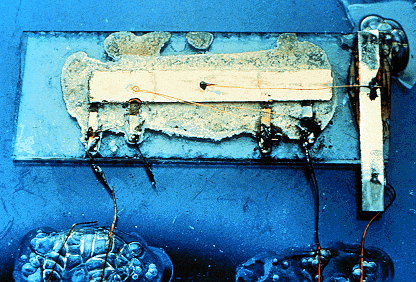
\includegraphics[scale=0.5]{./figures/C02-primer_circuito_integrado}
  \captionsetup{justification=centering}
  \caption{Primer circuito integrado presentado por Texas Instruments, Inc. el 
    12 de Septiembre de 1958}
  \label{fig:C02-primer_circuito_integrado}
\end{figure}

La ley de Moore, no es una ley en el sentido científico, sino más bien una
observación del ritmo de avance de la industria de aquellos momentos. Al momento
de publicar esas declaraciones, Moore trabajaba en los Laboratorios de Fairchild
Semiconductor, donde trabajaba junto a Robert Noyce. Ellos fueron los fundadores
de Intel en 1968. El ritmo de crecimiento de la insdustria de los
semiconductores dió lugar así, entre otras cosas, a la creación de los
microprocesadores.

\subsection{Microprocesadores}
\label{subsec:theory-history-microprocessor}

Los microprocesadores surgen como consecuencia del alto nivel de integración y
complejidad que la tencología de circuitos integrados permitieron alcanzar. Una
computadora digital, podía ser construída en uno o algunos pocos \emph{chips} de
circuitos integrados. Los primeros diseños de microprocesadores propiamente
dichos datan de fines de los años 60. Dentro de este contexto aparece el término
\emph{Central Processing Unit} (Unidad Central de Procesamiento) o CPU, que es
la parte de la máquina encargada de tomar los datos de entrada y las
intrucciones y generar los resultados, dentro del esquema del sistema de
procesamiento planteado al principio de éste capítulo. El microprocesador
integra además otros componentes y funcionalidades y se vale de ciertos
periféricos que pueden estar o no integrados en el mismo circuito, como por
ejemplo, memorias de sólo lectura (\emph{Read Only Memory} o ROM) y memorias de
acceso aleatorio (Random Access Memories o RAM) y dispositivos de
entrada/salida (\emph{I/O, input output devices}. El diseño de arquitecturas de
microprocesarores, como todo proceso de innovación tecnológica, no estuvo exento
de discusiones y distintas vertientes y prácticas a seguir. Los primeros diseños
de los que se tenga registro en órden cronológico, fueron:

\subsubsection{CADC}
\label{subsubsec:theory-history-microprocessor-cadc}

En 1968, la armada de los Estados Unidos de América le encomienda a la empresa
Garret AiResearch\footnote{Garret AiResearch: fundada en 1936 en Los Ángeles por
John Clifford ``Cliff'' Garret, fue una compañía dedicada  al desarrollo de
tecnologías relacionadas a la industria militar aérea.} la producción de una
computadora digital que pudiera competir con los sistemas electromecánicos que
estaban bajo desarrollo para los sistemas de control de vuelo del nuevo avión de
combate F-14 Tomcat. El diseño fue completado en 1970 y utilizaba un conjunto de
chips (\emph{chipset}) MOS como CPU, siendo aproximadamente 20 veces más pequeño
que su contraparte electromecánica y a su vez, mucho más confiable. Este diseño
fue utilizado en todos los primeros modelos de Tomcat. La armada se rehusó a
publicar el diseño hasta 1997, es por eso que la CADC (Central Air Data
Computer) y su \emph{chipset} asociado MP944 no son muy conocidos y no son
considerados en la mayoría de la bibliografía reelevante y es a partir de ese
momento en que son reconocidos como los primeros diseños válidos de
microprocesadores, y no sólo eso, si no que también son la primera especie de
\emph{Digital Signal Processor} (Procesador de Señales Digitales) o
DSP\footnote{``Digital Signal Processor'' (Procesaro de señales digitales): es
un tipo de microprocesador especializado en el tratamiento digital de señales}
puesto que además de las funciones de microprocesador, implementaba la
funcionalidad de medir variables como altitud, velocidad vertical y número de
\emph{mach} a partir de datos de sensores pitot, presión estática y temperatura.
Los responsables del diseño fueron Ray Holt y Steve Geller.

\begin{figure}
  \centering
  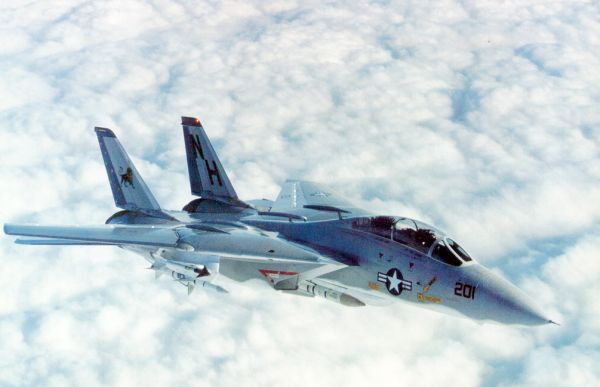
\includegraphics[scale=0.5]{./figures/C02-f14_tomcat}
  \captionsetup{justification=centering}
  \caption{Grumman F14 Tomcat, avión de combate de la US Navy cuyos sistemas de 
    vuelo eran controlados por la CADC.}
  \label{fig:C02-f14_tomcat}
\end{figure}


\subsubsection{Four-Phase Systems AL1}
\label{subsubsec:theory-history-microprocessor-al1}

Un diseño de Lee Boysel que data del año 1969 dentro de Texas
Instruments\footnote{Nota sobre TI}, era un componente de una implementación en
partes de un microprocesador de 24 bits, compuesto por tres chips iguales: AL1.
Durante un juicio por patentes, se demostró que una sóla AL1 junto con memorias
ROM y RAM e I/O era capaz de funcionar como CPU.

\begin{figure}
  \centering
  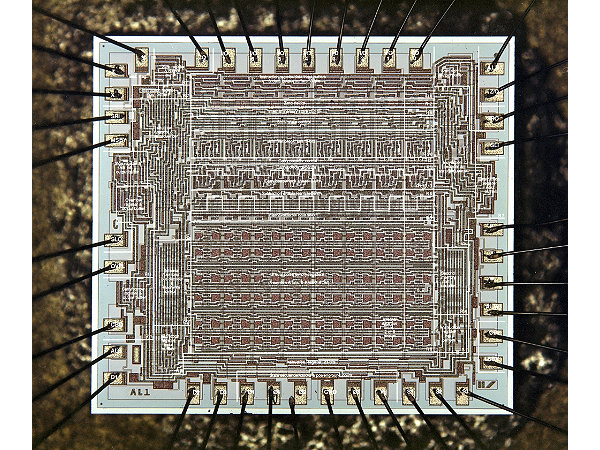
\includegraphics[scale=0.5]{./figures/C02-al1}
  \captionsetup{justification=centering}
  \caption{Imágen microscópica de la AL1 desarrollada por Four-Phase Systems 
    Inc..}
  \label{fig:C02-al1}
\end{figure}


\subsubsection{Pico/General Instruments}
\label{subsubsec:theory-history-microprocessor-pico-gi}

En 1971, Pico y General Instruments (GI) colaboraron en el diseño de circuitos
integrados con el objetivo de fabricar una implementación de un diseño de
\emph{chip} único para la calculadora Monroe/Litton Royal Digital III
Calcultator. Integraba en el mismo \emph{chip}, memoria ROM y RAM llamado
PICO1/GI250. Pico era un emprendimiento de cinco ingenieros de diseño de GI, que
tenían la visión de crear esta arquitectura en un único \emph{chip}. Contaban
con experiencia previa en diseños de \emph{chipsets} tanto de GI como de
Marconi-Elliot. Algunos de ellos habían trabajado para Elliot Automation para
crear una computadora de 8 bits en tecnología MOS, y habían ayudado a establecer
un laboratorio de investigación en tecnologías MOS en Escocia en el año 1967. El
mercado de las calculadoras estaba en pleno auge, con lo cuál estos diseños
supusieron un éxito comercial para Pico y GI. GI, por su parte continuó con la
innovación en microprocesadores  y microcontroladores y la división GI
Microelectronics se convirtió en 1987 en Microchip PIC Microcontroller.

\begin{figure}
  \centering
  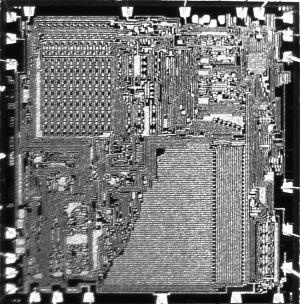
\includegraphics[scale=0.5]{./figures/C02-pico1_gi250}
  \captionsetup{justification=centering}
  \caption{Imágen microscópica del PICO1/GI250- Desarrollo colaborativo entre
    Pico y General Instruments de \emph{chip} único para la Monroe/Litton Royal 
    Digital III Calcultator.}
  \label{fig:C02-pico1_gi250}
\end{figure}

\subsubsection{Intel 4004}
\label{subsubsec:theory-history-microprocessor-4004}

El Intel 4004 es generalmente el reconocido como el primer microprocesador
comercial disponible en el mercado. El primer anuncio respecto de este
dispositivo data del 15 de Noviembre de 1971, en la publicación Electronic News.
El diseño nace a partir del requerimiento de una compañía japonesa fabricante de
calculadoras llamado Busicom, que le encomienda a Intel la tarea de desarrollar
un \emph{chipset} para calculadoras de escritorio de alto rendimiento. El diseño
original requerido por Busicom especificaba un \emph{chipset} compuesto por 7
\emph{chips} diferentes para la realización de una CPU de propósito específico
cuyo programa estuviera almacenado en una ROM y sus datos guardados memoria de
lectura y escritura implementada con registros de desplazamiento. Intel le
asignó el proyecto a Ted Hoff, quien propuso simplificar el diseño utilizando
almacenamiento en memoria RAM dinámica y una arquitectura de CPU de propósito
general. El diseño propuesto por Hoff implementaba la solución en 4
\emph{chips}: uno de ROM para almacenar el programa, uno de RAM dinámica para
almacenar los datos, un dispositivo sencillo de I/O y una CPU de 4 bits. A pesar
de no ser específicamente un diseñador de circuitos integrados, el supuso que se
podía integrar todo el CPU en un único \emph{chip}. Estas especificaciones
surgieron de la interacción de Hoff con un empleado a su cargo, el ingeniero de
software llamado Stanley Mazor y un ingeniero de Busicom llamado Masatoshi
Shima. Este proyecto se llamó MCS-4 y no fué hasta que Intel contratara al
italiano Federico Faggin que empezó a tomar su forma definitiva. Faggin venía de
desarollar en 1968 en Fairchild Semiconductor una teconología de compuertas de
silicio (SGT o \emph{Silicon Gate Technology}), técnica que se sigue aplicando
hoy en día. Faggin también era responsable del desarrollo de la técnica llamada
\emph{Random Logic} que permitió la síntesis de descripciones complejas de
lógica en hardware sencillo, como compuertas AND y OR. En el momento en el que
se estaba desarrollando el proyecto MCS-4, el responsable del área de diseño de
MOS de Intel era Leslie L. Vadász, cuya atención estaba enfocada en el mercado
de memorias. Fue gracias a esto que le otorgó el liderazgo del proyecto MCS-4 a
Faggin, quien fue finalmente el responsable de llevar el proyecto hasta la
concepción final del 4004 gracias a la aplicación de las técnicas de diseño y
fabricación antes mencionadas. Las primeras unidades del 4004 fueron entregadas
a Busicom en Marzo de 1971.

\begin{figure}
  \centering
  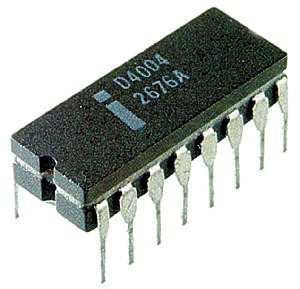
\includegraphics[scale=0.5]{./figures/C02-intel_4004}
  \captionsetup{justification=centering}
  \caption{Encapsulado del Intel 4004; que es considerado el primer
    microprocesador comercial en ser introducido en el mercado.}
  \label{fig:C02-intel_4004}
\end{figure}

\section{Evolución hacia las arquitecturas modernas}
\label{sec:theory-modern}

El concepto moderno de las arquitecturas se basa en las máquinas que almacenan
tanto el programa que se ejecuta, como los datos que se manjan en memoria de
lectura-escritura (\emph{Stored-Program digital computer}). Esto las diferencia
de las primeras implementaciones de los años 40, tales como
Colossus\footnote{Colossus era el nombre de una serie de computadoras
desarrolladas por los británicos para desencriptar las comunicaciones enemigas
durante la segunda guerra mundial. Implementadas con válvulas termoiónicas,
resolvían mediante lógica booleana operaciones de cálculo.} y la ENIAC.\\
En esta sección se estudian las distintas clasificaciones de arquitecturas
existentes hoy en día. Luego se detallarán diversas arquitecturas existentes y
se las enmarcará dentro de dichas clasificaciones.

\subsection{Clasificación de las arquitecturas según el acceso a la memoria de 
instrucciones y datos}
\label{subsec:theory-modern-memory_access}

Las instrucciones que ejecuta el procesador, al igual que los datos del programa
en ejecución, deben residir en la memoria. De este hecho se desprende que
existen ---al menos--- dos tipos de memorias: de instrucciones, y de datos. El
acceso a estas dos memorias puede realizarse a través del mismo
\emph{bus}\footnote{Bus: definir bus} o con \emph{buses} separados. Los nombres
que la historia les ha provisto a estos dos posibles enfoques, son
\emph{von Neumann} para las arquitecturas de \emph{bus} único y \emph{Harvard}
para aquellas de \emph{buses} separados.

\subsubsection{Arquitectura von Neumann}
\label{subsubsec:theory-modern-memory_access-von_neumann}

También conocida como modelo de von Neumann y arquitectura Princeton, este tipo
de arquitectura debe su nombre a John von Neumann\footnote{Nota sobre el
chango}, quién en el año 1945 describió en el documento inconcluso, cuya
carátula puede verse en la figura \ref{fig:C02-von_neumann_first_draft} y
conocido como \emph{First Draft of a Report on the EDVAC}\cite{vonNeumann}, una
arquitectura de computadora electrónica digital para ser implementada con
válvulas de vacío. Ésta fue la primera publicación dónde se describe el diseño
lógico de una computadora que utilizase el concepto de \emph{stored-program} o
programa almacenado. Este diseño, tal como fue llamado por el propio von
Neumann, \emph{very high speed automatic digital computing system} o sistema
automático digital de cómputo de muy alta velocidad, estaba dividido en 6
componentes:
\begin{itemize}
  \item CA: \emph{central arithmetic} o aritmética central
  \item CC: \emph{central control} o control central
  \item M: \emph{memory} o memoria
  \item I: \emph{input} o entrada
  \item O: \emph{output} o salida
  \item R: \emph{external memory} o memoria externa
\end{itemize}
\begin{figure}
  \centering
  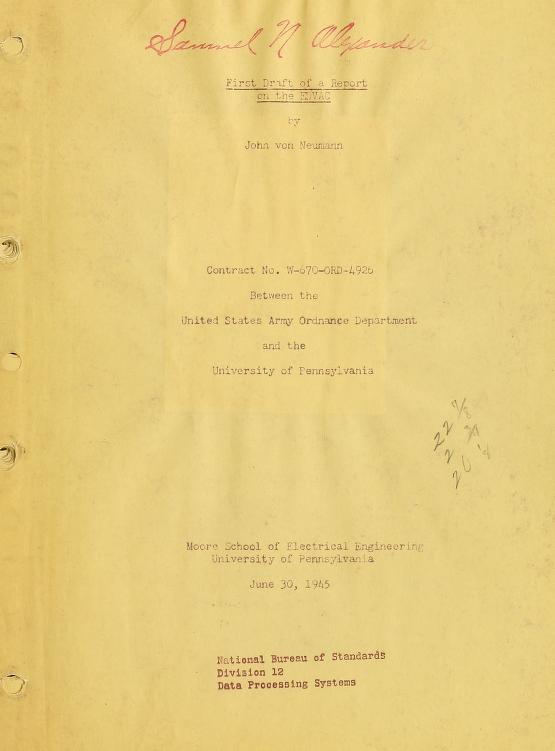
\includegraphics[scale=0.25]{./figures/C02-von_neumann_first_draft}
  \captionsetup{justification=centering}
  \caption{Carátula del escrito de von Neumann First Draft of a Report on the EDVAC}
  \label{fig:C02-von_neumann_first_draft}
\end{figure}
La memoria almacena tanto números (datos) como órdenes (instrucciones).
La aritmética central podía realizar sumas, restas, multiplicaciones, divisiones
y raices cuadradas. Otras operaciones matemáticas, como logaritmos y funciones
trigonométricas se debían realizar utilizando tablas de búsqueda e
interpolaciones, posiblemente bicuadráticas. Una decisión de diseño establecida
en el documento estableció que multiplicaciones y divisiones podían realizarse
mediante tablas logarítmicas, pero para poder mantener dichas tablas pequeñas
debería utilizarse interpolaciones, lo cuál a su vez necesita de
multiplicaciones, aunque de menor precisión.\\
Los números se represetaban mediante notación binaria. Estimó que 27 dígitos
binarios\footnote{En el documento se hace meción a dígitos binarios y no a
\emph{bits}, término que fue acuñado en 1948 por Claude Shannon} deberían ser
suficientes, pero redondéo a 30 dígitos, más uno de signo y otro para
diferenciar los números de las órdenes, resultando en palabras de 32 dígitos
binarios. La aritmética utilizada era complemento a dos para simplificar la
operación de resta. Para la multiplicación y la división, propuso ubicar el
punto binario luego del bit de signo, lo que implica que el dominio de los
operandos y resultados está en el rango -1 a 1, y por lo tanto, los datos y
resultados de los programas deberían ser escalados acordemente.\\
En cuanto al diseño de los circuitos, estableció que deberían utilizarse
válvulas de vacío, dejando de lado los relé, dada a la mayor velocidad provista
por las primeras. Otras sugerencias involucraban mantener al sistema de cómputo
lo más sencillo posible, evitando cualquier tipo de optimización de performance
mediante la superposición de operaciones. Las operaciones aritméticas debían
realizarse de a un dígito binario a la vez. Estimó el tiempo de la suma de dos
dígitos binarios en un microsegundo, por lo tanto la multiplicación de dos
números representados por 30 dígitos binarios deberí realizarse en
aproximadamente $30^{20}$ microsegundos; lo cuál era mucho más rápido que el
tiempo de cualquier dispositivo de cálculo del momento. El diseño estaba basado
en lo que von Neumann llamó ``elemento E'', basándose en el modelo biológico de
las neuronas, pero implementado de forma digital planteando que podrían ser
fabricados mediante una o dos válvulas. En términos modernos, la forma más
sencilla del ``elemento E'' es una compuerta \emph{AND} de dos entradas, con una
de sus entradas invertidas, llamada ``entrada de inhibición''. Al agregar más
entradas a este dispositivo, se establecía un nivel de umbral, el cual al ser
superado por la suma de una determinada cantidad de entradas generaba una salida
en tanto y en cuanto no se excitara la entrada de inhibición. También estableció
que dichos elementos de múltiples entradas podían ser construidos utilizando
combinaciones de la versión elemental, pero recomendaba implementarlos por
completo utilizando así menos válvulas de vacío con el objetivo de lograr
circuitos más sencillos y rápidos, principio que hoy en día se mantiene
vigente.\\
Toda función lógica arbitraria, podía implentarse, entonces, a partir de dichos
``elementos E''. Demostró en este trabajo, cómo implementar circuitos que
implementaban las funciones aritméticas, así como elementos de memoria y
circuitos de control, sin referirse en ningún momento al término de ``lógica
binaria''.\\
Los ciruitos debían ser sincrónicos, obteniendo la señal de reloj a partir de un
circuito oscilador implementado con válvulas y posiblemente controlado mediante
cristales osciladores. Los diagramas lógicos incluían los tiempos de demora
representados mediante una flecha. Estimó que la velocidad a la que se movía un
pulso eléctrico en un cable era de $300 mts/microsegundo$, por lo tanto no
debería generar problemas hasta obtener velocidades de reloj de $100MHz$.
Tambíen menciona pero no desarrolla la necesidad de contar con mecanismos de
detección y correción.\\
En cuanto a la memoria, que es donde entra la clasificación discutida en esta
sección, von Neumann estableció que la memoria es uniforme, conteniendo tanto
los números (datos) como las órdenes (instrucciones). Citando su trabajo:
\begin{quote}
  El dispositivo requiere una memoria considerable. A pesar de que pareciese 
  que distintas partes de la memoria tiene que realizar funciones que difieren 
  en su naturaleza y considerablemente en su propósito, resulta tentador tratar 
  a toda la memoria con un sólo órgano, y hacer que sus partes sean tan 
  intercambiables como sea posible para todas las funciones que deban realizar. 
  \cite[sección, 2.5]{vonNeumann}
\end{quote}
\begin{quote}
  Lás órdenes recibidas por CC vienen de M, es decir, el mismo lugar donde se
  almacenan los datos numéricos.\cite[sección, 14.0]{vonNeumann}.
\end{quote}
Él concluyó que la memoria sería el subsistema más grande y abarcativo de la
máquina. Basándose en diversos problemas matemáticos, incluyendo la resolución
de ecuaciones diferenciales parciales y ordinarias, ordenamientos y experimentos
probabilísticos, estimó que se necesitaba espacio para almacenar 8192 palabras
de 32 dígitos binarios para los datos, y algunos cientos de palabras para
almacenar las órdenes. Para la implementación de memoria, propuso dos tipos de
memoria rápida, \emph{delay line memory} e \emph{iconoscope}. Con estas
implementaciones planteó que la memoria debía ser direccionable por palabras y
para sortear los problemas de demora asociados a la lectura de estas memorias,
organizó las mismas en 256 conjuntos de 1024 dígitos binarios, o sea 32
palabras, logrando así direccionar los conjuntos con 8 dígitos binarios y las
palabras con 5 utilizando, entonces, 13 dígitos binarios en total para el
direccionamiento completo.\\
En su trabajo también estableció el formato de las órdenes, al cual llamó
``código''. Los tipos de órdenes incuyeron las operaciones aritméticas básicas,
así como el movimiento de palabras entre CA y M (análogas a las instrucciones
\emph{load} y \emph{store} de hoy en día que veremos más adelante), una órden
que elegía entre dos números basado en el signo del resultado de una operación
previa (análoga a una instrucción \emph{branch}), órdenes para controlar la
entrada y salida de datos y para indicarle a la CC que debía tomar instrucciones
desde otra sección de M (análoga a un \emph{jump}). Determinó, asimismo, la
cantidad de dígitos binarios necesarios para necesarios para los distintos tipos
de órdenes, sugirió lo que llamó ``órdenes inmediatas'', donde la siguiente
palabra  se trata del operando (lo cual también tiene una anagolía con ciertos
conjuntos de instrucciones actuales) y dejó planteado si era deseable dejar
dígitos sin especificar para propósitos futuros y mayor direccionamiento de
memoria.

\subsubsection{Arquitectura Harvard}
\label{subsubsec:theory-modern-memory_access-harvard}

Este tipo de arquitectura, ve sus orígenes en un desarrollo propuesto por el Dr.
Howard Aiken\footnote{Nota sobre Aiken} en la universidad de Harvard en el año
1937 basado en el trabajo llamado \emph{Analytical Engine}\footnote{Nota sobre
Analytical Engine} de Charles Babage\footnote{Nota sobre el tipo}. El desarrollo
fue llevado al cabo por IBM\footnote{Nota sobre IBM} y se trataba de una máquina
de cálculo llamada \emph{Automatic Sequence Controlled Calculator - Harvard Mark
I} entregado a la universidad el 24 de agosto de 1944. A diferencia de la
máquina propuesta (posteriormente) por von Neumann, ésta era una máquina
electromecánica construida con llaves, relés, engranajes y embreagues. Constaba
de 765000 componentes electromecánicos, cientos de millas de cableado, un peso
de 4.5 Ton. y un consumo de potencia de 3.7 kW. Para el ingreso de datos,
contaba con 60 conjuntos de 24 llaves rotativas que permitían ingresar números
decimales. Podía almacenar hast 72 números de hasta 23 dígitos decimales. En un
segundo era capaz de realizar 3 sumas o restas. La multiplicación tardaba 6
segundos y una división 13.5 segundos. El calculo de funciones logarítmicas o
trigonométricas utilizaba más de un minuto. Las instrucciones eran ingresadas a
través de cintas perforadas de 24 canales (en la figura
\ref{fig:C02-mark_i_instruction_tape} se puede ver una cinta con instrucciones
de esta máquina). Otra cinta podía ser utilizada para el ingreso de datos, pero
utilizando un formato distinto al de las instrucciones; estas no podían ser
ejecutadas desde los registros de almacenamiento. Esta separación entre datos e
instrucciones es lo que se conoce como arquitectura Harvard y que la diferencia
de la arquitectura von Neumann. El formato de las instrucciones definía tres
campos en ocho canales separados. Cada acumulador, cada conjunto de switches, y
los registros asociados a la entrada y salida y las unidades aritméticas tenían
asignado un índice único. Estos números eran representados en formato binario en
la cinta perforada de control, siendo el primer campo el índice del resultado de
la operación, el segundo el orígen del dato para la operación y el tercero el
código que representa la operación a realizar. Una particularidad de ésta
primera versión es que no tenía instrucción para el salto condicional en el
programa. Por lo tanto, los programas complejos debían ser largos y los
``loops'' se implementaban uniendo físicamente el final de la cinta perforada
del programa con el principio.\\
\begin{figure}
  \centering
  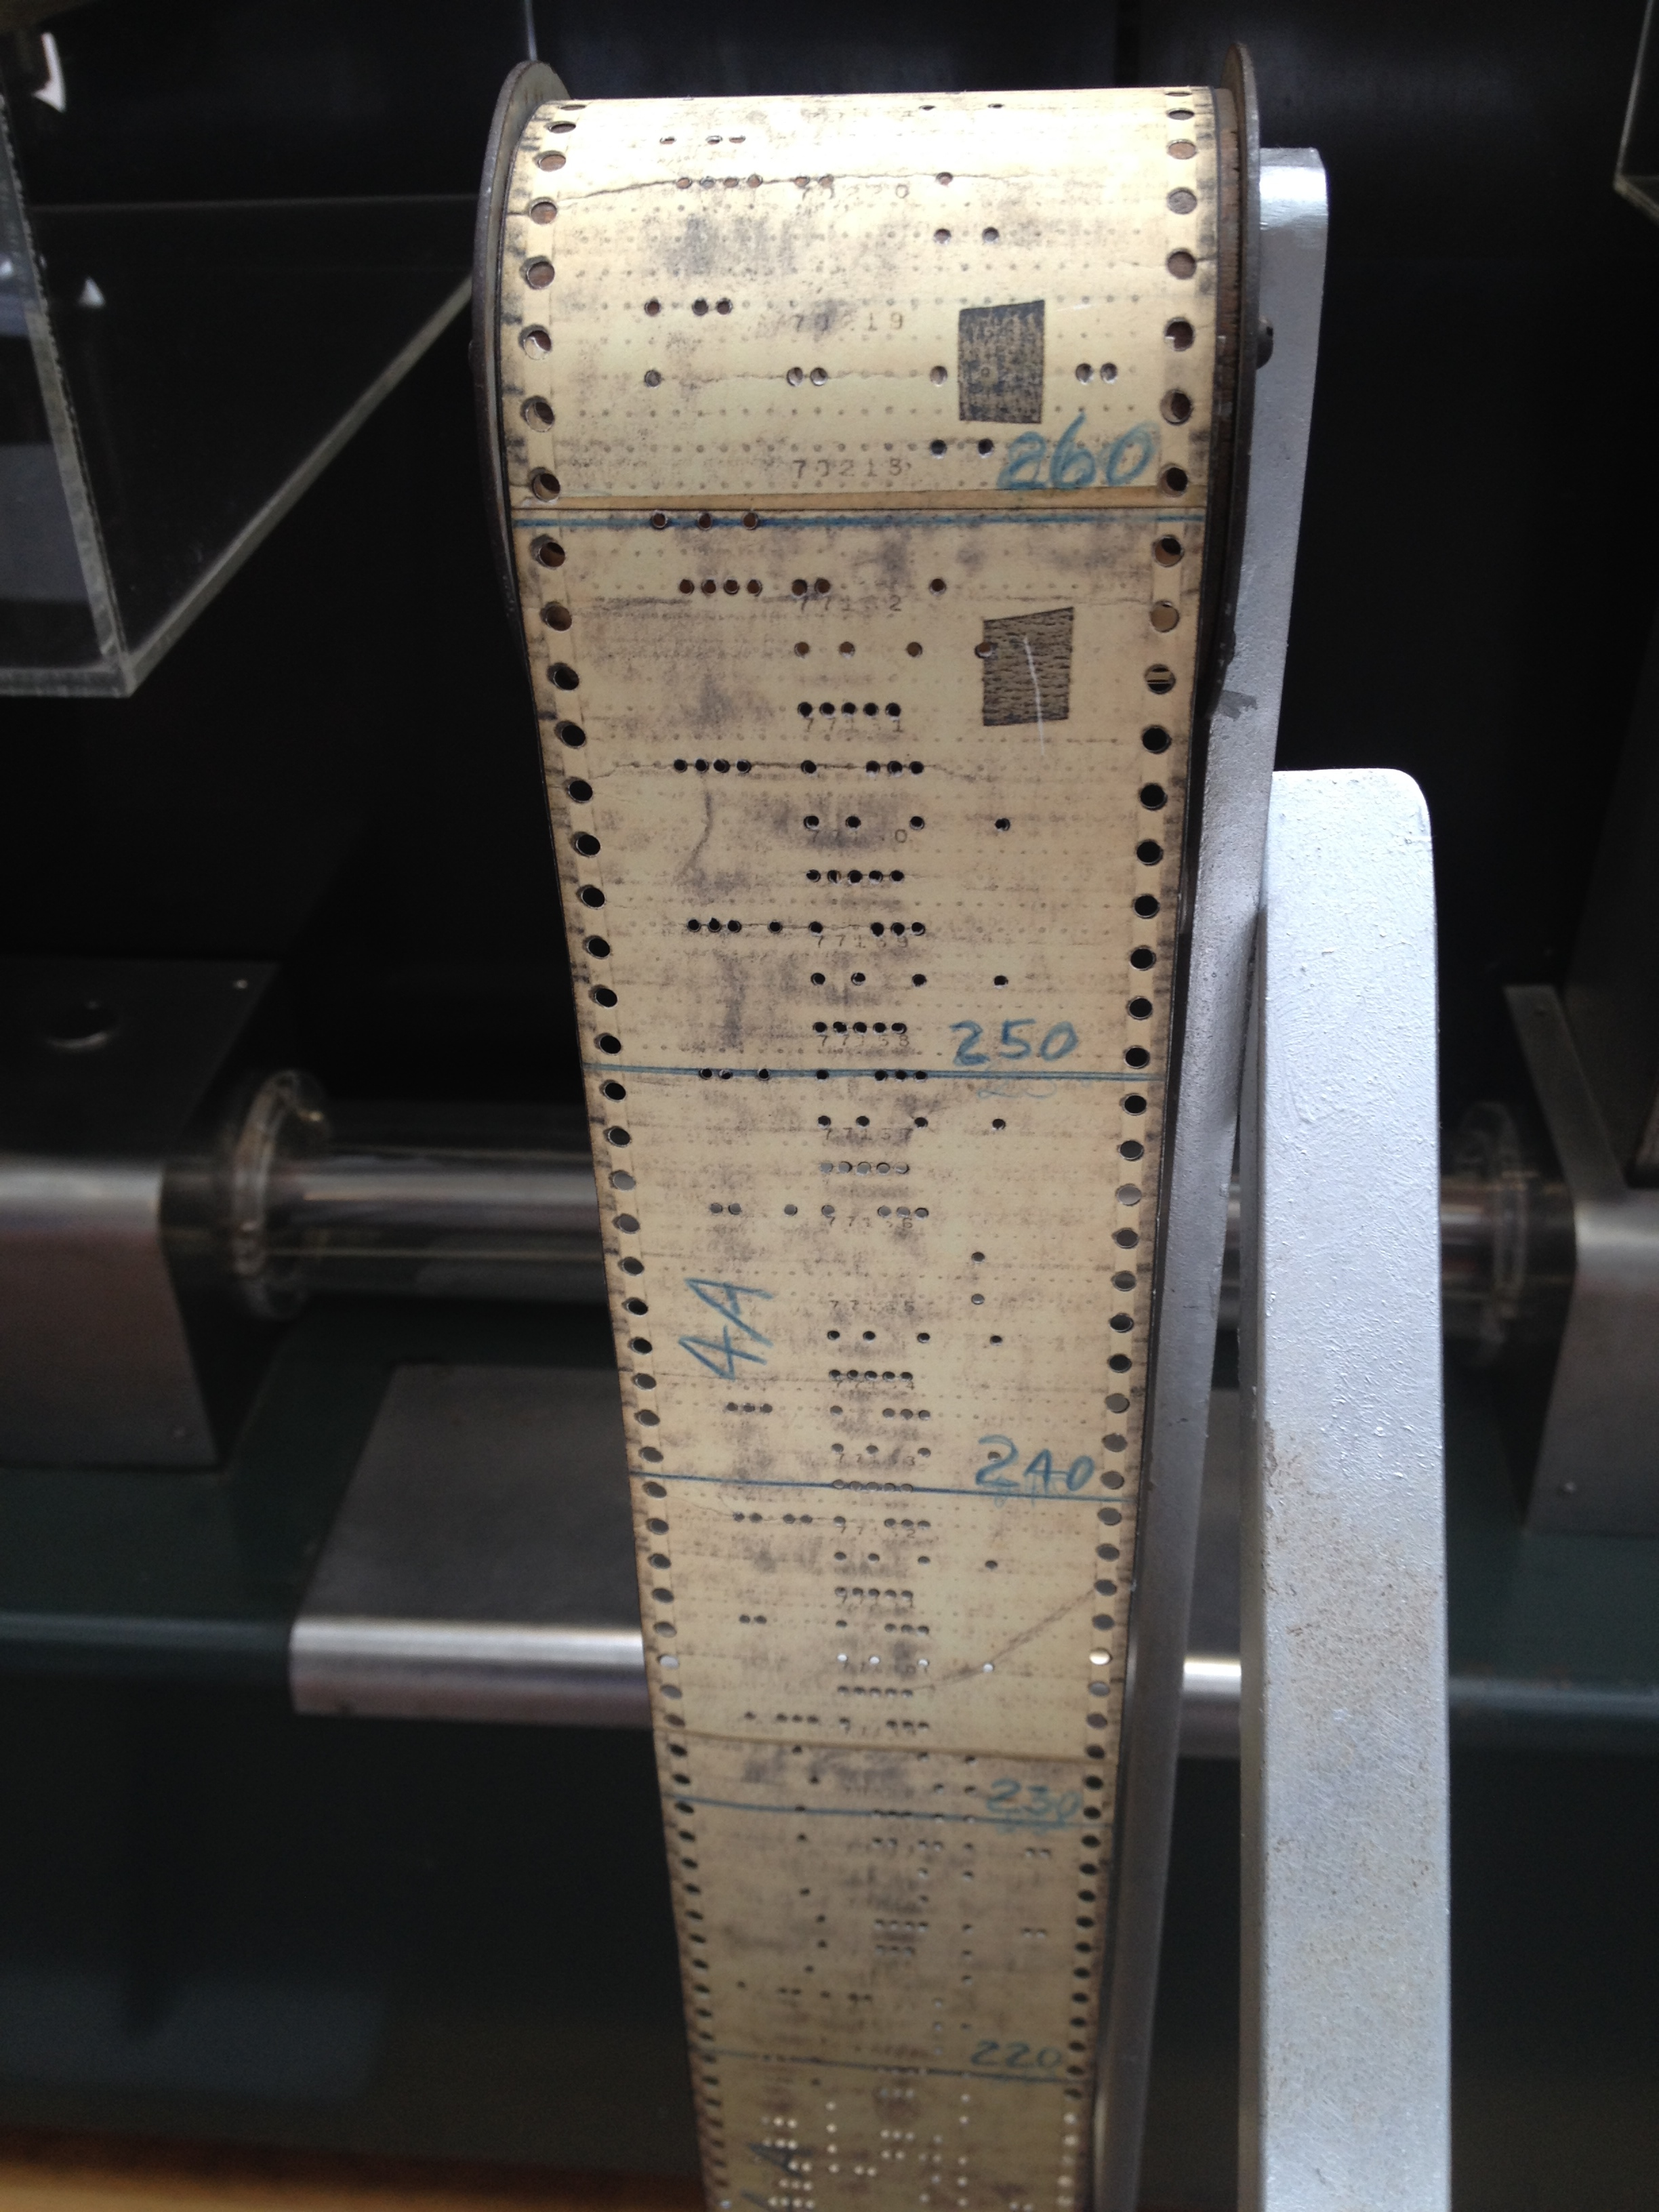
\includegraphics[scale=0.05]{./figures/C02-mark_i_instruction_tape}
  \captionsetup{justification=centering}
  \caption{Cinta de papel perforado con instrucciones de la Mark I}
  \label{fig:C02-mark_i_instruction_tape}
\end{figure}
La Mark I fue sucedida por la Mark II en el año 1948, la Mark III en septiembre
de 1949 y la Mark IV en el año 1952, todos estos proyectos fueron de Aiken. La
Mark II fue una mejora sobre la Mark I, pero aún basada en componentes
electromecánicos. La tercer versión utilizaba en su mayoría componentes
electrónicos tales como válvulas de vacío y diodos cristalinos, pero utilizaba
cilindros magnéticos para almacenamiento, y relés para la transferencia de datos
entre ellos. La cuarta versión fue la primera en ser completamente electrónica,
reemplazando los cilindros magnéticos de almacenamiento con memorias de núcle
magnético; el tipo de memoria de acceso aleatorio predominante entre 1955 y
1975.

\subsubsection{Harvard vs. von Neumann y Harvard modificada}
\label{subsubsec:theory-modern-memory_access-modified_harvard}

Como fue establecido al principio de esta sección, lo que diferencia estas dos
arquitecturas es el acceso a los datos y a las instrucciones. La arquitectura
von Neumann puede tratar a los datos como instrucciones y viceversa, dado que
para dicha arquitectura, la memoria es exactamente la misma, con el mismo tipo
de acceso y el mismo direccionamiento, contrariamente a lo que es una
arquitectura puramente Harvard, cuyas memorias de datos e instrucciones se
acceden por diferentes medios y cuyas direcciones pueden estar sobrepuestas (es
decir que la misma dirección de memoria no representa lo mismo si se trata de
datos o intrucciones) y por lo tanto, los datos y las intrucciones no pueden ser
intercambiados en el tratamiento que se realiza dentro de la unidad de cómputo.
Dadas estas condiciones, las principales desventajas son que, la arquitectura
von Neumann no puede acceder simultáneamente a datos y a instrucciones y la
máquina de Harvard no puede ni leer ni escribir en el espacio de memoria de las
instrucciones, denegando por lo tanto cualquier posibilidad de código
auto-optimizable o inteligente que reescriba sus instrucciones, así como tambíen
la carga de los programas a partir de medios de almacenamiento de datos.\\
Hoy en día, las máquinas puramente Harvard no son más que una especialidad.
Típicamente, en las máquinas modernas, se implementas arquitecturas Harvard
modificadas. Estas modificaciones pueden ser de diversos tipos:

\paragraph{Arquitectura de caché separado}
\label{par:theory-modern-memory_access-modified_harvard-split_cache}

Es la modificación más común sobre la arquitectura Harvard, se construye una
jerarquía de memoria donde el nivel más cercano al núcleo de procesamiento
(típicamente llamado caché de nivel 1) está separado en datos e instrucciones, y
unificando estas memorias en un nivel de jerarquía superior. Con esta técnia, se
puede relajar el problema de acceder a la memoria de instrucciones como datos,
tanto para la lectura como para la escritura al unificar toda la memoria en un
solo espacio de direccionamiento, emulando así el comportamiento de una
arquitectura de von Neumann, pero manteniendo la ventaja de poder acceder a
datos e instrucciones de forma simultánea. Esta característica será transparente
para la mayoría de los programadores, excepto aquellos casos en los que es
necesario el manejo de técnicas como por ejemplo, la coherencia de caches.

\paragraph{Acesso a instrucciones como datos}
\label{par:theory-modern-memory_access-modified_harvard-instructions_as_data}

Un arquitectura que provea esta solución matiene la naturaleza de espacios de
direcciones separados de la arquitectura Harvard, pero incluye operaciones
especializadas en acceder al contenido de la memoria de instrucciones como si
fueran datos. Como los datos no pueden ser ejecutados driectamente como
instrucciones, estas implementaciones no siempre son vistas como Harvard
``modificadas''.\\
Esta técnica puede presentarse con dos variantes. Por un lado, el acceso puede
ser de sólo lectura, provee la capacidad de copiar contenido embebido en el
código cargado en la memoria de instrucciones a la memoria de datos cuando el
programa comienza o, mejor aún, si los datos no van a cambiar (como es el caso
de constantes aritméticas o cadenas de texto predefinidas), estos datos que
están en la memoria de instrucciones pueden ser directamente leídos en tiempo de
ejecución por el programa sin tomar espacio de la memoria de datos (que puede
ser escasa en las implementaciones que aplican esta técnica). Por otro lado,
dicho acceso puede ser de lectura/escritura, suele darse cuando es necesaria una
capacidad de reprogramación de la máquina en cuestión. Pocas computadoras hoy en
día están basadas únicamente en ROM para su funcionamiento. Puede ser el caso de
algunos microcontroladores que tienen operaciones para escribir en su memoria
``Flash'' (en la cual se almacenan las instrucciones). Esta capacidad provee
medios de acceso para actualizaciones de software/firmware y reemplaza a las
EEPROM.

\paragraph{Ejecución de datos}
\label{par:theory-modern-memory_access-modified_harvard-data_execution}

Algunas arquitecturas pueden obtener sus instrucciones desde cualquier segmento
de memoria con la limitación de que no podrá acceder simultáneamente para leer
instrucciones y datos de un mismo segmento de memoria. Para lograr este
comportamiento, se direccionan los buses tanto de datos como de instrucciones
sobre distintos segmentos físicos de una misma memoria.

\paragraph{Características de las arquitecturas Harvard modificadas}
\label{par:theory-modern-memory_access-modified_harvard-characteristitcs}

Tres características pueden ser utilizadas para diferenciar a este tipo de
arquitectura de las Harvard puras y de las von Neumann:\\

\subparagraph{Las memorias de datos e instrucciones ocupan diferentes espacios
de direccionamiento}
\label{subpar:theory-modern-memory_access-modified_harvard-characteristitcs-1}

Para las máquinas puramente Harvard, hay una dirección ``cero'' de instrucciones
en el espacio de direcciones de las instrucciones y una dirección ``cero'' de
datos en el espacio de direcciones de los datos que referencian a un lugares de
almacenamiento distintos. En contraste, las máquinas von Neumann y algunas
Harvard modificadas (como las de caché separado), almacenan tanto datos como
instrucciones en un espacio de direcciones unificado, por lo tanto, la dirección
``cero'' hace referencia a una sóla cosa y lo almacenado allí puede ser la
representación binaria de un código de instrucción o de un dato, dependiendo de
cómo fue escrito el programa en ejecución. Sin embargo, tal como las máquinas
puramente Harvard, las Harvard modificadas con espacios de direcciones
separados, pero con instrucciones específicas que permiten leer y escribir las
instrucciones como datos, tienen una direcciónes solapadas para los respectivos
espacios de direccionamiento, por lo tanto esto no distingue las máquinas
puramente Harvard de este último tipo de Harvard modificadas.

\subparagraph{Las memorias de datos e instrucciones tienen conexiones físicas
separadas hacia el núcleo de procesamiento}
\label{subpar:theory-modern-memory_access-modified_harvard-characteristitcs-2}

Este es el motivo principal por el que existen las arquitecturas Harvard (tanto
puras como modificadas), y por qué coexisten con las más generales y flexibles
von Neumann: los caminos separados físicamente para los datos y las
instrucciones permiten que las instrucciones sean cargadas en la unidad de
cómputo al mismo tiempo que los datos, aumentando así el rendimiento. Las
máquinas puramente Harvard tienen caminos separados con espacios de direcciones
separados. Las máquinas de caché separado proveen este acceso separado para la
unidad de procesamiento pero presentan un espacio de direccionamiento unificado
al ascender en la jerarquía de memoria. Una máquina von Neumann puede tenera
sólamente un espacio de direcciones unificado. Para el punto de vista del
programador, una arquitectura de cache separado es tratada de forma equivalente
a una von Neumann (al menos hasta el punto en el que el tratamiendo de
coherencia de cache se convierta en significativo), como puede ser el caso de
código auto-optimizable o la carga de un programa en memoria desde un medio de
almacenamiento externo. Otras arquitecturas Harvard modificadas se comportan
como Harvard puras en este ámbito.

\subparagraph{Las memorias de datos e instrucciones pueden ser accedidas de
diferentes formas}
\label{subpar:theory-modern-memory_access-modified_harvard-characteristitcs-3}

Las máquinas Harvard puras, al tener distintos espacios de memoria para datos e
instrucciones, pueden acceder a dichas memorias de distintas maneras. Puede ser
el caso de una arquitectura donde la memoria de instrucciones se direccione con
una cantidad de bits distinta a la de datos. Esto no es posible en una
arquitectura von Neumann ni en una Harvard modificada de cache separado, dado
que ambos espacios de memoria deben estar superpuestos.

\subsubsection{Aplicaciones de esta clasificación en la actualidad}
\label{subsubsec:theory-modern-memory_access-current_aplications}

En áreas específicas donde un memoria cache es prohibitiva (puede ser el caso de
los DSP por el determinismo necesario para las diversas operaciones, o de
microcontroladores por el bajo costo), pueden darse arquitecturas Harvard puras
o von Neumann. En modelos donde el uso es de propósito general, típicamente se
utilizan arquitecturas Harvard modificadas con caché separado debido a que tener
espacios de direccionamiento separados genera dificultados con ciertos lenguajes
de programación de alto nivel que no soportan la noción de tener datos de sólo
lectura cargados en un espacio de direccionamiento distinto al de los datos
comunes, con la necesidad de utilizar distintas instrucciones para leerlos. El
lenguaje de programación ``C'' soporta este comportamiento a través de
extensiones propietarias, aunque hoy en día ya existen estandarizaciones para
los llamados procesares embebidos.

\subsection{Taxonomía de Flynn}
\label{subsec:theory-modern-flynn_taxonomy}

La taxonomía de Flynn es una clasificación de las arquitecturas basada en la 
cantidad de ``hilos'' de control y de datos que soporta el 
procesador de forma concurrente. Establecida en 1966 por Michael 
Flynn\footnote{Michael J. Flynn (Nacido el 20 de Mayo de 1934): es un profesor 
emérito de la universidad de Stanford que propuso la llamada ``Taxonomía de 
Flynn'' para clasificar las arquitecturas de computadoras en el año 1966}, 
estableciendo los efectos que pueden surgir de explotar el paralelismo tanto en 
los hilos de instrucciones como en los de datos. Se puede tener hilos únicos o 
múltiples para cada uno de ellos. Es estas definiciones, Flynn estableció que 
una máquina identifica los siguientes conceptos:
\begin{itemize}
  \item CU: \emph{contro unit} o unidad de control
  \item PE: \emph{processing element} o elemento de procesamiento
  \item IS: \emph{instruction stream} o hilo de instrucciones
  \item DS: \emph{data stream} o hilo de datos  
\end{itemize}
Al combinar hilos sencillos y múltiples de datos e instrucciones se da lugar, 
entonces, a cuatro tipo de arquitecturas (ver tabla \ref{tbl:flynn_taxonomy}).
\begin{table}
  \begin{tabu} to \textwidth {X[l]cc}
    \toprule
				& Hilo simple de instrucciones	& Hilo múltiple 
de instrucciones\\
    \midrule
    Hilo simple de datos	& SISD				& MISD\\
    Hilo múltiple de datos	& SIMD				& MIMD\\
    \bottomrule
  \end{tabu}
  \caption{Taxonomía de Flynn}
  \label{tbl:flynn_taxonomy}
\end{table}

\subsubsection{SISD: Simple Instruction stream, Simple Data stream}
\label{subsubsec:theory-modern-flynn_taxonomy-SISD}

Resultante de combinar un único hilo de control con un único hilo de datos, 
este tipo de arquitectura no explota ningún paralelismo en una máquina 
completamente secuencial. Una única CU obtiene un único IS de 
memoria. La CU genera las señales de control necesarias para excitar a un 
único PE sobre un único DS, es decir, una operación a la vez. Ver figura 
\ref{subfig:sisd}.\\
Un ejemplo de esta arquitectura son los procesadores de las antiguas 
computadoras personales.

\subsubsection{SIMD: Simple Instruction stream, Multiple Data stream}
\label{subsubsec:theory-modern-flynn_taxonomy-SIMD}

En este tipo de arquitecturas, sige existiendo un único hilo de control, pero 
los datos que afectan las instrucciones provienen de distintos hilos de datos. 
La CU trabaja con las instrucciones de un único IS y general las señales de 
control necesarias para que mútiples PE procesen los datos provenientes de 
múltiples DS. Es un tipo de máquina que es naturalmente paralelizable. Ver 
figura \ref{subfig:simd}.\\
Ejemplos de este tipo de arquitecturas son los procesadores matriciales y las 
unidades de procesamiento gráficas (GPU). Cabe destacar que los antiguos 
procesadores de PC, en un determinado momento incorporaron instrucciones 
específicas con el que lograban este comportamiento, tales como las extensiones 
multimedia (MMX) que Intel incluyó en su línea de procesadores Pentium a 
mediados de los años '90.

\subsubsection{MISD: Múltiple Instruction stream, Simple Data stream}
\label{subsubsec:theory-modern-flynn_taxonomy-MISD}

Se trata de arquitecturas en el que diversos hilos de control actuan sobre un 
único hilo de datos. No se trata de un tipo común de arquitecturas, si no más 
bien de un tipo específico utilizado en sistemas tolerantes a fallas. Diversos 
sistemas heterogéneos operan sobre el mismo hilo de datos y deben arribar al 
mismo resultado. Es decir que diversas CU toman instrucciones de diversos IS 
controlando múltiples PE que actuan sobre un único DS. Ver figura 
\ref{subfig:misd}.\\
Ejemplos de este tipo de máquinas pueden ser las computadoras de control de 
vuelo de aeronaves y naves espaciales o cohetes; es decir aplicaciones de 
misión crítica que poseen sistemas redundantes y decisores.

\subsubsection{MIMD: Multiple Instruction stream, Multiple Data stream}
\label{subsubsec:theory-modern-flynn_taxonomy-MIMD}

Se trata de arquitecturas donde múltiples procesadores simultáneamente ejecutan 
diversos hilos de instrucciones sobre diversos hilos de datos. Es decir que 
diversas CU toman instrucciones de diversos IS para excitar a diversos PE que 
actúan sobre diversos DS. Ver figura \ref{subfig:mimd}.\\
Los procesadores multinúcleo y los sistemas distribuidos son ejemplos de éste 
tipo de máquinas, y pueden utilizar tanto un espacio de memoria compartido, así 
como uno distribuído.
% TODO: Revisar por qué las últimas dos figuras no quedan bien armadas.
\begin{figure}
  \begin{subfigure}[b]{0.5\textwidth}
    % Graphic for TeX using PGF
% Title: /home/lnatale/Documents/xfire/digital/xfire_core/docs/thesis/tesis/figures/C02-sisd.dia
% Creator: Dia v0.97.3
% CreationDate: Sat Jul 23 17:44:13 2016
% For: lnatale
% \usepackage{tikz}
% The following commands are not supported in PSTricks at present
% We define them conditionally, so when they are implemented,
% this pgf file will use them.
\ifx\du\undefined
  \newlength{\du}
\fi
\setlength{\du}{15\unitlength}
\begin{tikzpicture}
\pgftransformxscale{1.000000}
\pgftransformyscale{-1.000000}
\definecolor{dialinecolor}{rgb}{0.000000, 0.000000, 0.000000}
\pgfsetstrokecolor{dialinecolor}
\definecolor{dialinecolor}{rgb}{1.000000, 1.000000, 1.000000}
\pgfsetfillcolor{dialinecolor}
\definecolor{dialinecolor}{rgb}{1.000000, 1.000000, 1.000000}
\pgfsetfillcolor{dialinecolor}
\fill (3.000000\du,2.000000\du)--(3.000000\du,4.000000\du)--(12.000000\du,4.000000\du)--(12.000000\du,2.000000\du)--cycle;
\pgfsetlinewidth{0.100000\du}
\pgfsetdash{}{0pt}
\pgfsetdash{}{0pt}
\pgfsetmiterjoin
\definecolor{dialinecolor}{rgb}{0.000000, 0.000000, 0.000000}
\pgfsetstrokecolor{dialinecolor}
\draw (3.000000\du,2.000000\du)--(3.000000\du,4.000000\du)--(12.000000\du,4.000000\du)--(12.000000\du,2.000000\du)--cycle;
% setfont left to latex
\definecolor{dialinecolor}{rgb}{0.000000, 0.000000, 0.000000}
\pgfsetstrokecolor{dialinecolor}
\node at (7.500000\du,3.195000\du){IS};
\definecolor{dialinecolor}{rgb}{1.000000, 1.000000, 1.000000}
\pgfsetfillcolor{dialinecolor}
\fill (0.000000\du,5.000000\du)--(0.000000\du,14.000000\du)--(2.000000\du,14.000000\du)--(2.000000\du,5.000000\du)--cycle;
\pgfsetlinewidth{0.100000\du}
\pgfsetdash{}{0pt}
\pgfsetdash{}{0pt}
\pgfsetmiterjoin
\definecolor{dialinecolor}{rgb}{0.000000, 0.000000, 0.000000}
\pgfsetstrokecolor{dialinecolor}
\draw (0.000000\du,5.000000\du)--(0.000000\du,14.000000\du)--(2.000000\du,14.000000\du)--(2.000000\du,5.000000\du)--cycle;
% setfont left to latex
\definecolor{dialinecolor}{rgb}{0.000000, 0.000000, 0.000000}
\pgfsetstrokecolor{dialinecolor}
\node at (1.000000\du,9.695000\du){DS};
% setfont left to latex
\definecolor{dialinecolor}{rgb}{0.000000, 0.000000, 0.000000}
\pgfsetstrokecolor{dialinecolor}
\node[anchor=west] at (1.000000\du,9.500000\du){};
% setfont left to latex
\definecolor{dialinecolor}{rgb}{0.000000, 0.000000, 0.000000}
\pgfsetstrokecolor{dialinecolor}
\node[anchor=west] at (7.500000\du,3.000000\du){};
\definecolor{dialinecolor}{rgb}{1.000000, 1.000000, 1.000000}
\pgfsetfillcolor{dialinecolor}
\fill (4.000000\du,8.000000\du)--(4.000000\du,11.000000\du)--(5.952500\du,11.000000\du)--(5.952500\du,8.000000\du)--cycle;
\pgfsetlinewidth{0.100000\du}
\pgfsetdash{}{0pt}
\pgfsetdash{}{0pt}
\pgfsetmiterjoin
\definecolor{dialinecolor}{rgb}{0.000000, 0.000000, 0.000000}
\pgfsetstrokecolor{dialinecolor}
\draw (4.000000\du,8.000000\du)--(4.000000\du,11.000000\du)--(5.952500\du,11.000000\du)--(5.952500\du,8.000000\du)--cycle;
% setfont left to latex
\definecolor{dialinecolor}{rgb}{0.000000, 0.000000, 0.000000}
\pgfsetstrokecolor{dialinecolor}
\node at (4.976250\du,9.695000\du){PE};
\pgfsetlinewidth{0.100000\du}
\pgfsetdash{}{0pt}
\pgfsetdash{}{0pt}
\pgfsetbuttcap
{
\definecolor{dialinecolor}{rgb}{0.000000, 0.000000, 0.000000}
\pgfsetfillcolor{dialinecolor}
% was here!!!
\pgfsetarrowsend{latex}
\definecolor{dialinecolor}{rgb}{0.000000, 0.000000, 0.000000}
\pgfsetstrokecolor{dialinecolor}
\draw (2.000000\du,9.500000\du)--(4.000000\du,9.500000\du);
}
\pgfsetlinewidth{0.100000\du}
\pgfsetdash{}{0pt}
\pgfsetdash{}{0pt}
\pgfsetmiterjoin
\pgfsetbuttcap
{
\definecolor{dialinecolor}{rgb}{0.000000, 0.000000, 0.000000}
\pgfsetfillcolor{dialinecolor}
% was here!!!
\pgfsetarrowsend{latex}
{\pgfsetcornersarced{\pgfpoint{0.000000\du}{0.000000\du}}\definecolor{dialinecolor}{rgb}{0.000000, 0.000000, 0.000000}
\pgfsetstrokecolor{dialinecolor}
\draw (7.500000\du,4.000000\du)--(10.000000\du,4.000000\du)--(10.000000\du,9.500000\du)--(5.952500\du,9.500000\du);
}}
% setfont left to latex
\definecolor{dialinecolor}{rgb}{0.000000, 0.000000, 0.000000}
\pgfsetstrokecolor{dialinecolor}
\node[anchor=west] at (4.976250\du,9.500000\du){};
\end{tikzpicture}

    \caption{SISD}
    \label{subfig:sisd}
  \end{subfigure}
  \begin{subfigure}[b]{0.5\textwidth}
    % Graphic for TeX using PGF
% Title: /home/lnatale/Documents/xfire/digital/xfire_core/docs/thesis/tesis/figures/C02-simd.dia
% Creator: Dia v0.97.3
% CreationDate: Mon Jul 25 12:32:33 2016
% For: lnatale
% \usepackage{tikz}
% The following commands are not supported in PSTricks at present
% We define them conditionally, so when they are implemented,
% this pgf file will use them.
\ifx\du\undefined
  \newlength{\du}
\fi
\setlength{\du}{15\unitlength}
\begin{tikzpicture}
\pgftransformxscale{1.000000}
\pgftransformyscale{-1.000000}
\definecolor{dialinecolor}{rgb}{0.000000, 0.000000, 0.000000}
\pgfsetstrokecolor{dialinecolor}
\definecolor{dialinecolor}{rgb}{1.000000, 1.000000, 1.000000}
\pgfsetfillcolor{dialinecolor}
\definecolor{dialinecolor}{rgb}{1.000000, 1.000000, 1.000000}
\pgfsetfillcolor{dialinecolor}
\fill (3.000000\du,2.000000\du)--(3.000000\du,4.000000\du)--(12.000000\du,4.000000\du)--(12.000000\du,2.000000\du)--cycle;
\pgfsetlinewidth{0.100000\du}
\pgfsetdash{}{0pt}
\pgfsetdash{}{0pt}
\pgfsetmiterjoin
\definecolor{dialinecolor}{rgb}{0.000000, 0.000000, 0.000000}
\pgfsetstrokecolor{dialinecolor}
\draw (3.000000\du,2.000000\du)--(3.000000\du,4.000000\du)--(12.000000\du,4.000000\du)--(12.000000\du,2.000000\du)--cycle;
% setfont left to latex
\definecolor{dialinecolor}{rgb}{0.000000, 0.000000, 0.000000}
\pgfsetstrokecolor{dialinecolor}
\node at (7.500000\du,3.195000\du){IS};
\definecolor{dialinecolor}{rgb}{1.000000, 1.000000, 1.000000}
\pgfsetfillcolor{dialinecolor}
\fill (0.000000\du,5.000000\du)--(0.000000\du,14.000000\du)--(2.000000\du,14.000000\du)--(2.000000\du,5.000000\du)--cycle;
\pgfsetlinewidth{0.100000\du}
\pgfsetdash{}{0pt}
\pgfsetdash{}{0pt}
\pgfsetmiterjoin
\definecolor{dialinecolor}{rgb}{0.000000, 0.000000, 0.000000}
\pgfsetstrokecolor{dialinecolor}
\draw (0.000000\du,5.000000\du)--(0.000000\du,14.000000\du)--(2.000000\du,14.000000\du)--(2.000000\du,5.000000\du)--cycle;
% setfont left to latex
\definecolor{dialinecolor}{rgb}{0.000000, 0.000000, 0.000000}
\pgfsetstrokecolor{dialinecolor}
\node at (1.000000\du,9.695000\du){DS};
% setfont left to latex
\definecolor{dialinecolor}{rgb}{0.000000, 0.000000, 0.000000}
\pgfsetstrokecolor{dialinecolor}
\node[anchor=west] at (1.000000\du,9.500000\du){};
% setfont left to latex
\definecolor{dialinecolor}{rgb}{0.000000, 0.000000, 0.000000}
\pgfsetstrokecolor{dialinecolor}
\node[anchor=west] at (7.500000\du,3.000000\du){};
\definecolor{dialinecolor}{rgb}{1.000000, 1.000000, 1.000000}
\pgfsetfillcolor{dialinecolor}
\fill (6.032827\du,5.000000\du)--(6.032827\du,7.000000\du)--(7.985327\du,7.000000\du)--(7.985327\du,5.000000\du)--cycle;
\pgfsetlinewidth{0.100000\du}
\pgfsetdash{}{0pt}
\pgfsetdash{}{0pt}
\pgfsetmiterjoin
\definecolor{dialinecolor}{rgb}{0.000000, 0.000000, 0.000000}
\pgfsetstrokecolor{dialinecolor}
\draw (6.032827\du,5.000000\du)--(6.032827\du,7.000000\du)--(7.985327\du,7.000000\du)--(7.985327\du,5.000000\du)--cycle;
% setfont left to latex
\definecolor{dialinecolor}{rgb}{0.000000, 0.000000, 0.000000}
\pgfsetstrokecolor{dialinecolor}
\node at (7.009077\du,6.195000\du){PE};
\pgfsetlinewidth{0.100000\du}
\pgfsetdash{}{0pt}
\pgfsetdash{}{0pt}
\pgfsetbuttcap
{
\definecolor{dialinecolor}{rgb}{0.000000, 0.000000, 0.000000}
\pgfsetfillcolor{dialinecolor}
% was here!!!
\pgfsetarrowsend{latex}
\definecolor{dialinecolor}{rgb}{0.000000, 0.000000, 0.000000}
\pgfsetstrokecolor{dialinecolor}
\draw (2.038676\du,6.001168\du)--(6.032827\du,6.000000\du);
}
% setfont left to latex
\definecolor{dialinecolor}{rgb}{0.000000, 0.000000, 0.000000}
\pgfsetstrokecolor{dialinecolor}
\node[anchor=west] at (7.009077\du,6.000000\du){};
\definecolor{dialinecolor}{rgb}{1.000000, 1.000000, 1.000000}
\pgfsetfillcolor{dialinecolor}
\fill (6.032827\du,8.563427\du)--(6.032827\du,10.463427\du)--(7.985327\du,10.463427\du)--(7.985327\du,8.563427\du)--cycle;
\pgfsetlinewidth{0.100000\du}
\pgfsetdash{}{0pt}
\pgfsetdash{}{0pt}
\pgfsetmiterjoin
\definecolor{dialinecolor}{rgb}{0.000000, 0.000000, 0.000000}
\pgfsetstrokecolor{dialinecolor}
\draw (6.032827\du,8.563427\du)--(6.032827\du,10.463427\du)--(7.985327\du,10.463427\du)--(7.985327\du,8.563427\du)--cycle;
% setfont left to latex
\definecolor{dialinecolor}{rgb}{0.000000, 0.000000, 0.000000}
\pgfsetstrokecolor{dialinecolor}
\node at (7.009077\du,9.708427\du){PE};
\definecolor{dialinecolor}{rgb}{1.000000, 1.000000, 1.000000}
\pgfsetfillcolor{dialinecolor}
\fill (6.032827\du,11.982323\du)--(6.032827\du,13.982323\du)--(7.985327\du,13.982323\du)--(7.985327\du,11.982323\du)--cycle;
\pgfsetlinewidth{0.100000\du}
\pgfsetdash{}{0pt}
\pgfsetdash{}{0pt}
\pgfsetmiterjoin
\definecolor{dialinecolor}{rgb}{0.000000, 0.000000, 0.000000}
\pgfsetstrokecolor{dialinecolor}
\draw (6.032827\du,11.982323\du)--(6.032827\du,13.982323\du)--(7.985327\du,13.982323\du)--(7.985327\du,11.982323\du)--cycle;
% setfont left to latex
\definecolor{dialinecolor}{rgb}{0.000000, 0.000000, 0.000000}
\pgfsetstrokecolor{dialinecolor}
\node at (7.009077\du,13.177323\du){PE};
\pgfsetlinewidth{0.100000\du}
\pgfsetdash{}{0pt}
\pgfsetdash{}{0pt}
\pgfsetbuttcap
{
\definecolor{dialinecolor}{rgb}{0.000000, 0.000000, 0.000000}
\pgfsetfillcolor{dialinecolor}
% was here!!!
\pgfsetarrowsend{latex}
\definecolor{dialinecolor}{rgb}{0.000000, 0.000000, 0.000000}
\pgfsetstrokecolor{dialinecolor}
\draw (2.049939\du,9.502801\du)--(6.032827\du,9.513427\du);
}
\pgfsetlinewidth{0.100000\du}
\pgfsetdash{}{0pt}
\pgfsetdash{}{0pt}
\pgfsetbuttcap
{
\definecolor{dialinecolor}{rgb}{0.000000, 0.000000, 0.000000}
\pgfsetfillcolor{dialinecolor}
% was here!!!
\pgfsetarrowsend{latex}
\definecolor{dialinecolor}{rgb}{0.000000, 0.000000, 0.000000}
\pgfsetstrokecolor{dialinecolor}
\draw (2.038676\du,12.994748\du)--(6.032827\du,12.982323\du);
}
\pgfsetlinewidth{0.100000\du}
\pgfsetdash{}{0pt}
\pgfsetdash{}{0pt}
\pgfsetmiterjoin
\pgfsetbuttcap
{
\definecolor{dialinecolor}{rgb}{0.000000, 0.000000, 0.000000}
\pgfsetfillcolor{dialinecolor}
% was here!!!
\pgfsetarrowsend{latex}
{\pgfsetcornersarced{\pgfpoint{0.000000\du}{0.000000\du}}\definecolor{dialinecolor}{rgb}{0.000000, 0.000000, 0.000000}
\pgfsetstrokecolor{dialinecolor}
\draw (7.500000\du,4.000000\du)--(10.043428\du,4.000000\du)--(10.043428\du,6.000000\du)--(7.985327\du,6.000000\du);
}}
\pgfsetlinewidth{0.100000\du}
\pgfsetdash{}{0pt}
\pgfsetdash{}{0pt}
\pgfsetmiterjoin
\pgfsetbuttcap
{
\definecolor{dialinecolor}{rgb}{0.000000, 0.000000, 0.000000}
\pgfsetfillcolor{dialinecolor}
% was here!!!
\pgfsetarrowsend{latex}
{\pgfsetcornersarced{\pgfpoint{0.000000\du}{0.000000\du}}\definecolor{dialinecolor}{rgb}{0.000000, 0.000000, 0.000000}
\pgfsetstrokecolor{dialinecolor}
\draw (7.500000\du,4.000000\du)--(10.047487\du,4.000000\du)--(10.047487\du,9.513427\du)--(7.985327\du,9.513427\du);
}}
\pgfsetlinewidth{0.100000\du}
\pgfsetdash{}{0pt}
\pgfsetdash{}{0pt}
\pgfsetmiterjoin
\pgfsetbuttcap
{
\definecolor{dialinecolor}{rgb}{0.000000, 0.000000, 0.000000}
\pgfsetfillcolor{dialinecolor}
% was here!!!
\pgfsetarrowsend{latex}
{\pgfsetcornersarced{\pgfpoint{0.000000\du}{0.000000\du}}\definecolor{dialinecolor}{rgb}{0.000000, 0.000000, 0.000000}
\pgfsetstrokecolor{dialinecolor}
\draw (7.500000\du,4.000000\du)--(10.053249\du,4.000000\du)--(10.053249\du,12.982323\du)--(7.985327\du,12.982323\du);
}}
\end{tikzpicture}

    \caption{SIMD}
    \label{subfig:simd}
  \end{subfigure}
  \begin{subfigure}[b]{0.5\textwidth}
    % Graphic for TeX using PGF
% Title: /home/lnatale/Documents/xfire/digital/xfire_core/docs/thesis/tesis/figures/C02-misd.dia
% Creator: Dia v0.97.3
% CreationDate: Mon Jul 25 12:58:01 2016
% For: lnatale
% \usepackage{tikz}
% The following commands are not supported in PSTricks at present
% We define them conditionally, so when they are implemented,
% this pgf file will use them.
\ifx\du\undefined
  \newlength{\du}
\fi
\setlength{\du}{15\unitlength}
\begin{tikzpicture}
\pgftransformxscale{1.000000}
\pgftransformyscale{-1.000000}
\definecolor{dialinecolor}{rgb}{0.000000, 0.000000, 0.000000}
\pgfsetstrokecolor{dialinecolor}
\definecolor{dialinecolor}{rgb}{1.000000, 1.000000, 1.000000}
\pgfsetfillcolor{dialinecolor}
\definecolor{dialinecolor}{rgb}{1.000000, 1.000000, 1.000000}
\pgfsetfillcolor{dialinecolor}
\fill (3.000000\du,2.000000\du)--(3.000000\du,4.000000\du)--(12.000000\du,4.000000\du)--(12.000000\du,2.000000\du)--cycle;
\pgfsetlinewidth{0.100000\du}
\pgfsetdash{}{0pt}
\pgfsetdash{}{0pt}
\pgfsetmiterjoin
\definecolor{dialinecolor}{rgb}{0.000000, 0.000000, 0.000000}
\pgfsetstrokecolor{dialinecolor}
\draw (3.000000\du,2.000000\du)--(3.000000\du,4.000000\du)--(12.000000\du,4.000000\du)--(12.000000\du,2.000000\du)--cycle;
% setfont left to latex
\definecolor{dialinecolor}{rgb}{0.000000, 0.000000, 0.000000}
\pgfsetstrokecolor{dialinecolor}
\node at (7.500000\du,3.195000\du){IS};
\definecolor{dialinecolor}{rgb}{1.000000, 1.000000, 1.000000}
\pgfsetfillcolor{dialinecolor}
\fill (0.000000\du,5.000000\du)--(0.000000\du,14.000000\du)--(2.000000\du,14.000000\du)--(2.000000\du,5.000000\du)--cycle;
\pgfsetlinewidth{0.100000\du}
\pgfsetdash{}{0pt}
\pgfsetdash{}{0pt}
\pgfsetmiterjoin
\definecolor{dialinecolor}{rgb}{0.000000, 0.000000, 0.000000}
\pgfsetstrokecolor{dialinecolor}
\draw (0.000000\du,5.000000\du)--(0.000000\du,14.000000\du)--(2.000000\du,14.000000\du)--(2.000000\du,5.000000\du)--cycle;
% setfont left to latex
\definecolor{dialinecolor}{rgb}{0.000000, 0.000000, 0.000000}
\pgfsetstrokecolor{dialinecolor}
\node at (1.000000\du,9.695000\du){DS};
% setfont left to latex
\definecolor{dialinecolor}{rgb}{0.000000, 0.000000, 0.000000}
\pgfsetstrokecolor{dialinecolor}
\node[anchor=west] at (1.000000\du,9.500000\du){};
% setfont left to latex
\definecolor{dialinecolor}{rgb}{0.000000, 0.000000, 0.000000}
\pgfsetstrokecolor{dialinecolor}
\node[anchor=west] at (7.500000\du,3.000000\du){};
% setfont left to latex
\definecolor{dialinecolor}{rgb}{0.000000, 0.000000, 0.000000}
\pgfsetstrokecolor{dialinecolor}
\node[anchor=west] at (7.009080\du,6.000000\du){};
\definecolor{dialinecolor}{rgb}{1.000000, 1.000000, 1.000000}
\pgfsetfillcolor{dialinecolor}
\fill (3.266103\du,8.552919\du)--(3.266103\du,10.452919\du)--(5.218603\du,10.452919\du)--(5.218603\du,8.552919\du)--cycle;
\pgfsetlinewidth{0.100000\du}
\pgfsetdash{}{0pt}
\pgfsetdash{}{0pt}
\pgfsetmiterjoin
\definecolor{dialinecolor}{rgb}{0.000000, 0.000000, 0.000000}
\pgfsetstrokecolor{dialinecolor}
\draw (3.266103\du,8.552919\du)--(3.266103\du,10.452919\du)--(5.218603\du,10.452919\du)--(5.218603\du,8.552919\du)--cycle;
% setfont left to latex
\definecolor{dialinecolor}{rgb}{0.000000, 0.000000, 0.000000}
\pgfsetstrokecolor{dialinecolor}
\node at (4.242353\du,9.697919\du){PE};
\definecolor{dialinecolor}{rgb}{1.000000, 1.000000, 1.000000}
\pgfsetfillcolor{dialinecolor}
\fill (8.148914\du,8.547671\du)--(8.148914\du,10.447671\du)--(10.101414\du,10.447671\du)--(10.101414\du,8.547671\du)--cycle;
\pgfsetlinewidth{0.100000\du}
\pgfsetdash{}{0pt}
\pgfsetdash{}{0pt}
\pgfsetmiterjoin
\definecolor{dialinecolor}{rgb}{0.000000, 0.000000, 0.000000}
\pgfsetstrokecolor{dialinecolor}
\draw (8.148914\du,8.547671\du)--(8.148914\du,10.447671\du)--(10.101414\du,10.447671\du)--(10.101414\du,8.547671\du)--cycle;
% setfont left to latex
\definecolor{dialinecolor}{rgb}{0.000000, 0.000000, 0.000000}
\pgfsetstrokecolor{dialinecolor}
\node at (9.125164\du,9.692671\du){PE};
\pgfsetlinewidth{0.100000\du}
\pgfsetdash{}{0pt}
\pgfsetdash{}{0pt}
\pgfsetbuttcap
{
\definecolor{dialinecolor}{rgb}{0.000000, 0.000000, 0.000000}
\pgfsetfillcolor{dialinecolor}
% was here!!!
\pgfsetarrowsend{latex}
\definecolor{dialinecolor}{rgb}{0.000000, 0.000000, 0.000000}
\pgfsetstrokecolor{dialinecolor}
\draw (2.049511\du,9.501352\du)--(3.266103\du,9.502919\du);
}
\pgfsetlinewidth{0.100000\du}
\pgfsetdash{}{0pt}
\pgfsetdash{}{0pt}
\pgfsetmiterjoin
\pgfsetbuttcap
{
\definecolor{dialinecolor}{rgb}{0.000000, 0.000000, 0.000000}
\pgfsetfillcolor{dialinecolor}
% was here!!!
\pgfsetarrowsend{latex}
{\pgfsetcornersarced{\pgfpoint{0.000000\du}{0.000000\du}}\definecolor{dialinecolor}{rgb}{0.000000, 0.000000, 0.000000}
\pgfsetstrokecolor{dialinecolor}
\draw (7.500000\du,4.000000\du)--(6.394405\du,4.000000\du)--(6.394405\du,9.502919\du)--(5.218603\du,9.502919\du);
}}
\pgfsetlinewidth{0.100000\du}
\pgfsetdash{}{0pt}
\pgfsetdash{}{0pt}
\pgfsetmiterjoin
\pgfsetbuttcap
{
\definecolor{dialinecolor}{rgb}{0.000000, 0.000000, 0.000000}
\pgfsetfillcolor{dialinecolor}
% was here!!!
\pgfsetarrowsend{latex}
{\pgfsetcornersarced{\pgfpoint{0.000000\du}{0.000000\du}}\definecolor{dialinecolor}{rgb}{0.000000, 0.000000, 0.000000}
\pgfsetstrokecolor{dialinecolor}
\draw (7.500000\du,4.000000\du)--(11.167340\du,4.000000\du)--(11.167340\du,9.497671\du)--(10.101414\du,9.497671\du);
}}
\pgfsetlinewidth{0.100000\du}
\pgfsetdash{}{0pt}
\pgfsetdash{}{0pt}
\pgfsetmiterjoin
\pgfsetbuttcap
{
\definecolor{dialinecolor}{rgb}{0.000000, 0.000000, 0.000000}
\pgfsetfillcolor{dialinecolor}
% was here!!!
\pgfsetarrowsend{latex}
{\pgfsetcornersarced{\pgfpoint{0.000000\du}{0.000000\du}}\definecolor{dialinecolor}{rgb}{0.000000, 0.000000, 0.000000}
\pgfsetstrokecolor{dialinecolor}
\draw (2.000000\du,9.500000\du)--(2.389020\du,9.500796\du)--(2.385419\du,7.549235\du)--(6.852144\du,7.548144\du)--(6.852042\du,9.497842\du)--(8.148914\du,9.497671\du);
}}
\end{tikzpicture}

    \caption{MISD}
    \label{subfig:misd}
  \end{subfigure}
  \begin{subfigure}[b]{0.5\textwidth}
    % Graphic for TeX using PGF
% Title: /home/lnatale/Documents/xfire/digital/xfire_core/docs/thesis/tesis/figures/C02-mimd.dia
% Creator: Dia v0.97.3
% CreationDate: Mon Jul 25 13:04:08 2016
% For: lnatale
% \usepackage{tikz}
% The following commands are not supported in PSTricks at present
% We define them conditionally, so when they are implemented,
% this pgf file will use them.
\ifx\du\undefined
  \newlength{\du}
\fi
\setlength{\du}{15\unitlength}
\begin{tikzpicture}
\pgftransformxscale{1.000000}
\pgftransformyscale{-1.000000}
\definecolor{dialinecolor}{rgb}{0.000000, 0.000000, 0.000000}
\pgfsetstrokecolor{dialinecolor}
\definecolor{dialinecolor}{rgb}{1.000000, 1.000000, 1.000000}
\pgfsetfillcolor{dialinecolor}
\definecolor{dialinecolor}{rgb}{1.000000, 1.000000, 1.000000}
\pgfsetfillcolor{dialinecolor}
\fill (3.000000\du,2.000000\du)--(3.000000\du,4.000000\du)--(12.000000\du,4.000000\du)--(12.000000\du,2.000000\du)--cycle;
\pgfsetlinewidth{0.100000\du}
\pgfsetdash{}{0pt}
\pgfsetdash{}{0pt}
\pgfsetmiterjoin
\definecolor{dialinecolor}{rgb}{0.000000, 0.000000, 0.000000}
\pgfsetstrokecolor{dialinecolor}
\draw (3.000000\du,2.000000\du)--(3.000000\du,4.000000\du)--(12.000000\du,4.000000\du)--(12.000000\du,2.000000\du)--cycle;
% setfont left to latex
\definecolor{dialinecolor}{rgb}{0.000000, 0.000000, 0.000000}
\pgfsetstrokecolor{dialinecolor}
\node at (7.500000\du,3.195000\du){IS};
\definecolor{dialinecolor}{rgb}{1.000000, 1.000000, 1.000000}
\pgfsetfillcolor{dialinecolor}
\fill (0.000000\du,5.000000\du)--(0.000000\du,14.000000\du)--(2.000000\du,14.000000\du)--(2.000000\du,5.000000\du)--cycle;
\pgfsetlinewidth{0.100000\du}
\pgfsetdash{}{0pt}
\pgfsetdash{}{0pt}
\pgfsetmiterjoin
\definecolor{dialinecolor}{rgb}{0.000000, 0.000000, 0.000000}
\pgfsetstrokecolor{dialinecolor}
\draw (0.000000\du,5.000000\du)--(0.000000\du,14.000000\du)--(2.000000\du,14.000000\du)--(2.000000\du,5.000000\du)--cycle;
% setfont left to latex
\definecolor{dialinecolor}{rgb}{0.000000, 0.000000, 0.000000}
\pgfsetstrokecolor{dialinecolor}
\node at (1.000000\du,9.695000\du){DS};
% setfont left to latex
\definecolor{dialinecolor}{rgb}{0.000000, 0.000000, 0.000000}
\pgfsetstrokecolor{dialinecolor}
\node[anchor=west] at (1.000000\du,9.500000\du){};
% setfont left to latex
\definecolor{dialinecolor}{rgb}{0.000000, 0.000000, 0.000000}
\pgfsetstrokecolor{dialinecolor}
\node[anchor=west] at (7.500000\du,3.000000\du){};
% setfont left to latex
\definecolor{dialinecolor}{rgb}{0.000000, 0.000000, 0.000000}
\pgfsetstrokecolor{dialinecolor}
\node[anchor=west] at (7.009080\du,6.000000\du){};
\definecolor{dialinecolor}{rgb}{1.000000, 1.000000, 1.000000}
\pgfsetfillcolor{dialinecolor}
\fill (3.266103\du,8.552919\du)--(3.266103\du,10.452919\du)--(5.218603\du,10.452919\du)--(5.218603\du,8.552919\du)--cycle;
\pgfsetlinewidth{0.100000\du}
\pgfsetdash{}{0pt}
\pgfsetdash{}{0pt}
\pgfsetmiterjoin
\definecolor{dialinecolor}{rgb}{0.000000, 0.000000, 0.000000}
\pgfsetstrokecolor{dialinecolor}
\draw (3.266103\du,8.552919\du)--(3.266103\du,10.452919\du)--(5.218603\du,10.452919\du)--(5.218603\du,8.552919\du)--cycle;
% setfont left to latex
\definecolor{dialinecolor}{rgb}{0.000000, 0.000000, 0.000000}
\pgfsetstrokecolor{dialinecolor}
\node at (4.242353\du,9.697919\du){PE};
\definecolor{dialinecolor}{rgb}{1.000000, 1.000000, 1.000000}
\pgfsetfillcolor{dialinecolor}
\fill (8.148914\du,8.547671\du)--(8.148914\du,10.447671\du)--(10.101414\du,10.447671\du)--(10.101414\du,8.547671\du)--cycle;
\pgfsetlinewidth{0.100000\du}
\pgfsetdash{}{0pt}
\pgfsetdash{}{0pt}
\pgfsetmiterjoin
\definecolor{dialinecolor}{rgb}{0.000000, 0.000000, 0.000000}
\pgfsetstrokecolor{dialinecolor}
\draw (8.148914\du,8.547671\du)--(8.148914\du,10.447671\du)--(10.101414\du,10.447671\du)--(10.101414\du,8.547671\du)--cycle;
% setfont left to latex
\definecolor{dialinecolor}{rgb}{0.000000, 0.000000, 0.000000}
\pgfsetstrokecolor{dialinecolor}
\node at (9.125164\du,9.692671\du){PE};
\pgfsetlinewidth{0.100000\du}
\pgfsetdash{}{0pt}
\pgfsetdash{}{0pt}
\pgfsetbuttcap
{
\definecolor{dialinecolor}{rgb}{0.000000, 0.000000, 0.000000}
\pgfsetfillcolor{dialinecolor}
% was here!!!
\pgfsetarrowsend{latex}
\definecolor{dialinecolor}{rgb}{0.000000, 0.000000, 0.000000}
\pgfsetstrokecolor{dialinecolor}
\draw (2.049511\du,9.501352\du)--(3.266103\du,9.502919\du);
}
\pgfsetlinewidth{0.100000\du}
\pgfsetdash{}{0pt}
\pgfsetdash{}{0pt}
\pgfsetmiterjoin
\pgfsetbuttcap
{
\definecolor{dialinecolor}{rgb}{0.000000, 0.000000, 0.000000}
\pgfsetfillcolor{dialinecolor}
% was here!!!
\pgfsetarrowsend{latex}
{\pgfsetcornersarced{\pgfpoint{0.000000\du}{0.000000\du}}\definecolor{dialinecolor}{rgb}{0.000000, 0.000000, 0.000000}
\pgfsetstrokecolor{dialinecolor}
\draw (7.500000\du,4.000000\du)--(6.394405\du,4.000000\du)--(6.394405\du,9.502919\du)--(5.218603\du,9.502919\du);
}}
\pgfsetlinewidth{0.100000\du}
\pgfsetdash{}{0pt}
\pgfsetdash{}{0pt}
\pgfsetmiterjoin
\pgfsetbuttcap
{
\definecolor{dialinecolor}{rgb}{0.000000, 0.000000, 0.000000}
\pgfsetfillcolor{dialinecolor}
% was here!!!
\pgfsetarrowsend{latex}
{\pgfsetcornersarced{\pgfpoint{0.000000\du}{0.000000\du}}\definecolor{dialinecolor}{rgb}{0.000000, 0.000000, 0.000000}
\pgfsetstrokecolor{dialinecolor}
\draw (7.500000\du,4.000000\du)--(11.167340\du,4.000000\du)--(11.167340\du,9.497671\du)--(10.101414\du,9.497671\du);
}}
\definecolor{dialinecolor}{rgb}{1.000000, 1.000000, 1.000000}
\pgfsetfillcolor{dialinecolor}
\fill (3.277406\du,11.949153\du)--(3.277406\du,13.849153\du)--(5.229906\du,13.849153\du)--(5.229906\du,11.949153\du)--cycle;
\pgfsetlinewidth{0.100000\du}
\pgfsetdash{}{0pt}
\pgfsetdash{}{0pt}
\pgfsetmiterjoin
\definecolor{dialinecolor}{rgb}{0.000000, 0.000000, 0.000000}
\pgfsetstrokecolor{dialinecolor}
\draw (3.277406\du,11.949153\du)--(3.277406\du,13.849153\du)--(5.229906\du,13.849153\du)--(5.229906\du,11.949153\du)--cycle;
% setfont left to latex
\definecolor{dialinecolor}{rgb}{0.000000, 0.000000, 0.000000}
\pgfsetstrokecolor{dialinecolor}
\node at (4.253656\du,13.094153\du){PE};
\definecolor{dialinecolor}{rgb}{1.000000, 1.000000, 1.000000}
\pgfsetfillcolor{dialinecolor}
\fill (8.160216\du,11.943906\du)--(8.160216\du,13.843906\du)--(10.112716\du,13.843906\du)--(10.112716\du,11.943906\du)--cycle;
\pgfsetlinewidth{0.100000\du}
\pgfsetdash{}{0pt}
\pgfsetdash{}{0pt}
\pgfsetmiterjoin
\definecolor{dialinecolor}{rgb}{0.000000, 0.000000, 0.000000}
\pgfsetstrokecolor{dialinecolor}
\draw (8.160216\du,11.943906\du)--(8.160216\du,13.843906\du)--(10.112716\du,13.843906\du)--(10.112716\du,11.943906\du)--cycle;
% setfont left to latex
\definecolor{dialinecolor}{rgb}{0.000000, 0.000000, 0.000000}
\pgfsetstrokecolor{dialinecolor}
\node at (9.136466\du,13.088906\du){PE};
\pgfsetlinewidth{0.100000\du}
\pgfsetdash{}{0pt}
\pgfsetdash{}{0pt}
\pgfsetbuttcap
{
\definecolor{dialinecolor}{rgb}{0.000000, 0.000000, 0.000000}
\pgfsetfillcolor{dialinecolor}
% was here!!!
\pgfsetarrowsend{latex}
\definecolor{dialinecolor}{rgb}{0.000000, 0.000000, 0.000000}
\pgfsetstrokecolor{dialinecolor}
\draw (2.060814\du,12.897586\du)--(3.277406\du,12.899153\du);
}
\pgfsetlinewidth{0.100000\du}
\pgfsetdash{}{0pt}
\pgfsetdash{}{0pt}
\pgfsetmiterjoin
\pgfsetbuttcap
{
\definecolor{dialinecolor}{rgb}{0.000000, 0.000000, 0.000000}
\pgfsetfillcolor{dialinecolor}
% was here!!!
\pgfsetarrowsend{latex}
{\pgfsetcornersarced{\pgfpoint{0.000000\du}{0.000000\du}}\definecolor{dialinecolor}{rgb}{0.000000, 0.000000, 0.000000}
\pgfsetstrokecolor{dialinecolor}
\draw (7.500000\du,4.000000\du)--(6.405708\du,4.000000\du)--(6.405708\du,12.899153\du)--(5.229906\du,12.899153\du);
}}
\pgfsetlinewidth{0.100000\du}
\pgfsetdash{}{0pt}
\pgfsetdash{}{0pt}
\pgfsetmiterjoin
\pgfsetbuttcap
{
\definecolor{dialinecolor}{rgb}{0.000000, 0.000000, 0.000000}
\pgfsetfillcolor{dialinecolor}
% was here!!!
\pgfsetarrowsend{latex}
{\pgfsetcornersarced{\pgfpoint{0.000000\du}{0.000000\du}}\definecolor{dialinecolor}{rgb}{0.000000, 0.000000, 0.000000}
\pgfsetstrokecolor{dialinecolor}
\draw (7.500000\du,4.000000\du)--(11.178643\du,4.000000\du)--(11.178643\du,12.893906\du)--(10.112716\du,12.893906\du);
}}
\definecolor{dialinecolor}{rgb}{1.000000, 1.000000, 1.000000}
\pgfsetfillcolor{dialinecolor}
\fill (3.278098\du,5.310896\du)--(3.278098\du,7.210896\du)--(5.230598\du,7.210896\du)--(5.230598\du,5.310896\du)--cycle;
\pgfsetlinewidth{0.100000\du}
\pgfsetdash{}{0pt}
\pgfsetdash{}{0pt}
\pgfsetmiterjoin
\definecolor{dialinecolor}{rgb}{0.000000, 0.000000, 0.000000}
\pgfsetstrokecolor{dialinecolor}
\draw (3.278098\du,5.310896\du)--(3.278098\du,7.210896\du)--(5.230598\du,7.210896\du)--(5.230598\du,5.310896\du)--cycle;
% setfont left to latex
\definecolor{dialinecolor}{rgb}{0.000000, 0.000000, 0.000000}
\pgfsetstrokecolor{dialinecolor}
\node at (4.254348\du,6.455896\du){PE};
\definecolor{dialinecolor}{rgb}{1.000000, 1.000000, 1.000000}
\pgfsetfillcolor{dialinecolor}
\fill (8.160908\du,5.305648\du)--(8.160908\du,7.205648\du)--(10.113408\du,7.205648\du)--(10.113408\du,5.305648\du)--cycle;
\pgfsetlinewidth{0.100000\du}
\pgfsetdash{}{0pt}
\pgfsetdash{}{0pt}
\pgfsetmiterjoin
\definecolor{dialinecolor}{rgb}{0.000000, 0.000000, 0.000000}
\pgfsetstrokecolor{dialinecolor}
\draw (8.160908\du,5.305648\du)--(8.160908\du,7.205648\du)--(10.113408\du,7.205648\du)--(10.113408\du,5.305648\du)--cycle;
% setfont left to latex
\definecolor{dialinecolor}{rgb}{0.000000, 0.000000, 0.000000}
\pgfsetstrokecolor{dialinecolor}
\node at (9.137158\du,6.450648\du){PE};
\pgfsetlinewidth{0.100000\du}
\pgfsetdash{}{0pt}
\pgfsetdash{}{0pt}
\pgfsetbuttcap
{
\definecolor{dialinecolor}{rgb}{0.000000, 0.000000, 0.000000}
\pgfsetfillcolor{dialinecolor}
% was here!!!
\pgfsetarrowsend{latex}
\definecolor{dialinecolor}{rgb}{0.000000, 0.000000, 0.000000}
\pgfsetstrokecolor{dialinecolor}
\draw (2.061506\du,6.259328\du)--(3.278098\du,6.260896\du);
}
\pgfsetlinewidth{0.100000\du}
\pgfsetdash{}{0pt}
\pgfsetdash{}{0pt}
\pgfsetmiterjoin
\pgfsetbuttcap
{
\definecolor{dialinecolor}{rgb}{0.000000, 0.000000, 0.000000}
\pgfsetfillcolor{dialinecolor}
% was here!!!
\pgfsetarrowsend{latex}
{\pgfsetcornersarced{\pgfpoint{0.000000\du}{0.000000\du}}\definecolor{dialinecolor}{rgb}{0.000000, 0.000000, 0.000000}
\pgfsetstrokecolor{dialinecolor}
\draw (7.500000\du,4.000000\du)--(6.406400\du,4.000000\du)--(6.406400\du,6.260896\du)--(5.230598\du,6.260896\du);
}}
\pgfsetlinewidth{0.100000\du}
\pgfsetdash{}{0pt}
\pgfsetdash{}{0pt}
\pgfsetmiterjoin
\pgfsetbuttcap
{
\definecolor{dialinecolor}{rgb}{0.000000, 0.000000, 0.000000}
\pgfsetfillcolor{dialinecolor}
% was here!!!
\pgfsetarrowsend{latex}
{\pgfsetcornersarced{\pgfpoint{0.000000\du}{0.000000\du}}\definecolor{dialinecolor}{rgb}{0.000000, 0.000000, 0.000000}
\pgfsetstrokecolor{dialinecolor}
\draw (7.500000\du,4.000000\du)--(11.179335\du,4.000000\du)--(11.179335\du,6.255648\du)--(10.113408\du,6.255648\du);
}}
\pgfsetlinewidth{0.100000\du}
\pgfsetdash{}{0pt}
\pgfsetdash{}{0pt}
\pgfsetmiterjoin
\pgfsetbuttcap
{
\definecolor{dialinecolor}{rgb}{0.000000, 0.000000, 0.000000}
\pgfsetfillcolor{dialinecolor}
% was here!!!
\pgfsetarrowsend{latex}
{\pgfsetcornersarced{\pgfpoint{0.000000\du}{0.000000\du}}\definecolor{dialinecolor}{rgb}{0.000000, 0.000000, 0.000000}
\pgfsetstrokecolor{dialinecolor}
\draw (2.049379\du,4.998826\du)--(6.857748\du,5.000656\du)--(6.856605\du,6.278116\du)--(8.153476\du,6.277945\du);
}}
\pgfsetlinewidth{0.100000\du}
\pgfsetdash{}{0pt}
\pgfsetdash{}{0pt}
\pgfsetmiterjoin
\pgfsetbuttcap
{
\definecolor{dialinecolor}{rgb}{0.000000, 0.000000, 0.000000}
\pgfsetfillcolor{dialinecolor}
% was here!!!
\pgfsetarrowsend{latex}
{\pgfsetcornersarced{\pgfpoint{0.000000\du}{0.000000\du}}\definecolor{dialinecolor}{rgb}{0.000000, 0.000000, 0.000000}
\pgfsetstrokecolor{dialinecolor}
\draw (2.033681\du,8.209392\du)--(6.842050\du,8.211222\du)--(6.840907\du,9.488682\du)--(8.137778\du,9.488511\du);
}}
\pgfsetlinewidth{0.100000\du}
\pgfsetdash{}{0pt}
\pgfsetdash{}{0pt}
\pgfsetmiterjoin
\pgfsetbuttcap
{
\definecolor{dialinecolor}{rgb}{0.000000, 0.000000, 0.000000}
\pgfsetfillcolor{dialinecolor}
% was here!!!
\pgfsetarrowsend{latex}
{\pgfsetcornersarced{\pgfpoint{0.000000\du}{0.000000\du}}\definecolor{dialinecolor}{rgb}{0.000000, 0.000000, 0.000000}
\pgfsetstrokecolor{dialinecolor}
\draw (2.041113\du,11.628238\du)--(6.849482\du,11.630068\du)--(6.848339\du,12.907528\du)--(8.145210\du,12.907357\du);
}}
\end{tikzpicture}

    \caption{MIMD}
    \label{subfig:mimd}
  \end{subfigure}
  \caption{Diagramas de la taxonomía de Flynn}
  \label{fig:flynn_taxonomy}
\end{figure}

\subsubsection{Actualización de la taxonomía de Flynn}
\label{subsubsec:theory-modern-flynn_taxonomy-today}

Con el advenimiento de las arquitecturas multinúcleo ---hoy en día la mayoría 
de las arquitecturas utilizadas en microprocesadores y microcontroladores son 
multinúcleo--- la taxonomía de Flynn ha recibido una actualización para la 
categoría MIMD, basándose en el programa al que pertenencen los hilos de datos 
e instrucciones en cuestión. Estos grupos son conocidos como ``Single Program, 
Multiple Data Streams'' (SPMD) y ``Multiple Programs, Multiple Data Streams'' 
(MPMD).

\paragraph{SPMD: Single Program, Multiple Data streams}
\label{par:theory-modern-flynn_taxonomy-today-SPMD}

Esta clasificación modela múltiples procesadores autónomos que simultánemente 
ejecutan el mismo programa (pero en punto independientes, a diferencia de la 
naturaleza secuencial de SIMD) en diversos hilos de datos del programa. En sí, 
no es sólo la naturaleza de la arquitectura lo que da lugar a este tipo, si no 
que además involucra al modelo de programación utilizado.

\paragraph{MPMD: Multiple Programs, Multiple Data streams}
\label{par:theory-modern-flynn_taxonomy-today-MPMD}

También se trata de un modelo que involucra tanto a la arquitectura como al 
diseño del software que se ejecuta. En este caso, múltiples procesadores 
ejectuan simultáneamente al menos dos programas independientes. Típicamente, 
estos sistemas eligen un nodo que administra como los demás nodos ejecutan el 
resto de los programas con diversas estrategias y modelos de programación.

\subsection{Clasificación de las arquitecturas según el manejo de los datos y 
cantidad de operandos}
\label{subsec:theory-modern-data_managment}

Tal como fuese indicado al comienzo del presente capítulo, la unidad de 
procesamiento, recibe datos e intrucciones y genera resultados. Para poder 
realizar este trabajo, la arquitectura debe ser capaz de leer de la memoria 
datos y luego volcar los resultados a la misma. En este proceso, hay diversos 
mecanismos por el cual las instrucciones pueden obtenera esta información y 
devolverla luego del procesamiento para un posterior uso en el programa o 
generar salidas en el sistema. Inherentemente, se definen la cantidad de 
operandos que pueden tener las instrucciones de la arquitectura.\\
Es así que las instrucciones de la arquitectura, podrían operar directamente 
sobre los datos en memoria y escribir los resultados en la misma; hacer uso de 
estructuras de hardware intermedias para almacenar los datos temporalmente para 
su procesamiento y posterior almacenamiento o una combinación de estas 
alternativas.\\
Las ventajas, desventajas y particualridades que presentará cada una de las 
variantes deben ser sopesadas con la tecnología de los compiladores utilizados 
y las posibilidades de optimización que proveen.\\
Previo a analizar las alternativas de diseño que se presentan en cuanto al 
manejo de los datos dentro de la unidad de procesamiento, es conveniete 
estudiar los diversos modos de direccionamiento que podemos observar en las 
arquitecturas a través de la historia.

\subsubsection{Modos de direccionamiento}
\label{subsubsec:theory-modern-data_managment-addressing_modes}

Las instrucciones deben ser capaces de entregarle datos o referencias a los 
mismos a la unidad de procesamiento. Así mismo, la unidad de procesamiento debe 
poder enviar los resultados a alguna salida. Estos mecanismos se conocen como 
modos de direccionamiento. Para el ingreso de datos, estos pueden estar 
embebidos en el código de la instrucción, pueden ser representados por su 
dirección en memoria o estar contenidos en algún registro interno. Para la 
salida, también podremos enviarlos a alguna dirección de meomoria representada 
de alguna manera en particular, o sencillamente almacenar el dato en algún 
registro interno.\\
No sólo son los datos los que deben ser direccionados para ingresar a la unidad 
de procesamiento; esta también debe ser capaz de obtener las instrucciones de 
memoria.\\
En el caso de las instrucciones, el direccionamiento cobra importancia al 
momento de analizar las instrucciones que modifican el flujo del programa y 
rompen con la secuencialidad del mismo, o sea las instrucciones de salto 
condicional e incondicional. Se reconocen principalmente tres variantes:
\begin{itemize}
  \item Absoluta o directa: el código de la instrucción lleva embebido 
directamente la dirección de la instrucción a la que se debe saltar.
  \item Relativa: el código de la instrucción lleva embebido un desplazamiento 
respecto de la dirección de la siguiente instrucción a ejecutar, siendo que ese 
desplazamiento puede ser en ambos sentidos.
  \item Indirecta: el código de la instrucción lleva embebido el registro que 
indica a qué dirección debe saltar la ejecución del programa.
\end{itemize}
Al analizar los posibles modos de direccionamiento de los datos, surgen más 
alternativas básicas:
\begin{itemize}
  \item Registro: es el utilizado en las operaciones en las cuales todos los 
operandos se obtienen y escriben desde registros internos.
  \item Desplazamiento: en este modo de direccionamiento las instrucciones que 
lo implementan indican la dirección de memoria a la cual acceder utilizando un 
como base una dirección contenida en un registro a la cual se le suma un 
desplazamiento que está embebido en la instrucción. Existen diversas variantes 
de este modo de direccionamiento, algunos de los cuales utilizan índices para 
recorrer estructuras de memoria más complejas.
  \item Inmediato: para este caso, la instrucción posee embebido en el código 
de la operación el dato.
  \item Implícito: las instrucciones que implementan este modo de 
direccionamiento sólamente actúan sobre algún dato específico dentro de algún 
registro interno.
\end{itemize}

\subsubsection{Accumulator}
\label{subsubsec:theory-modern-data_managment-accumulator}

Las arquitecturas Accumulator, o de acumulador, también llamadas máquinas de un 
operando, se caracterizan por tener un registro particular ---típicamente 
llamado acumulador--- en el que los resultados de las operaciones entre dicho 
registro y el operando indicado en la instrucción se almacena. El operando 
puede ser obtenido con los diversos modos de direccionamiento soportado por tal 
arquitectura.\\
Esta arquitectura basa su funcionamiento en el hecho de que en general, los 
programas realizan una secuencia de operaciones sobre los datos. Por lo tanto, 
si no existiese el acumulador, cada vez que se realiza una operación, se 
debería guardar el resultado en memoria, para luego volver a obtenerlo para 
seguir operando. Dado que la tecnología con la que se implementan los registros 
internos permiten mayor velocidad de transferencia que la memoria principal 
(más larga y más lenta pero de menor costo), se utiliza este registro especial 
para explotar la localidad temporal de los datos en el software.

\subsubsection{Stack}
\label{subsubsec:theory-modern-data_managment-stack}

La estructura ``stack'' o pila, es una estructura lógica que permite ir 
apilando y desapilando datos. En una arquitectura de tipo stack, existe este 
tipo de estructura implementada con registros internos y las operaciones se 
realizan entre los dos elementos superiores de la pila y el resultado se 
almacena al tope. Los datos utilizados son removidos del tope en el proceso. Es 
evidente la necesidad de instrucciones específicas (o posibles 
pseudoinstrucciones) para mover datos entre la pila y la memoria. En este 
escenario, también existirán diversos modos de direccionamiento para los datos. 
Típicamente, el conjunto de instrucciones notará las operaciones en RPN (Reverse 
Polish Notation)\footnote{Reverse Polish Notation (Notación Polaca Inversa): 
DESARROLLAR} y en el código de la operación se elimina la necesidad de 
explicitar los operandos. Una variación de esta arquitectura puede implementar 
operaciones entre el tope de pila y otro operando indicado en la instrucción 
mediante los diversos modos de direccionamiento soportados por tal 
implementación.\\
Esta arquitectura tal como la de acumulador también explota la localidad 
temporal de los datos considerando la secuencialidad de las operaciones sobre 
los mismos. De hecho, puede considerarse a la arquitectura acumulador como un 
caso especial de pila con un único registro que opera contra los operandos 
indicados en la instrucción.

\subsubsection{Load / Store}
\label{subsubsec:theory-modern-data_managment-load_store}

También conocidas como ``Register / Register'' estas arquitecturas 
implementan múltiples registros internos direccionables y sólo realizan 
operaciones entre ellos. Además se proveen instrucciones específicas de carga y 
almacenamiento para mover los datos entre memoria y los registros internos. 
Dichas instrucciones proveerán los diversos modos de direccionamiento de datos 
soportados por tal arquitectura.\\
En implementaciones de este tipo, se resigna por un lado las ventajas que 
presenta la localidad temporal de los datos en pos de explotar posibilidades 
del paralelismo a nivel de instrucción, que es tódo un tópico en sí mismo 
dentro de las optimizaciones posibles de las arquitecturas. Hoy en día, ésta es 
la elección clásica al momento de desarrollar una arquitectura RISC.

\subsubsection{Register / Memory}
\label{subsubsec:theory-modern-data_managment-register_memory}

Estas arquitecturas, como lo indica su nombre, permiten que las operaciones 
sean realizadas en o desde memoria, así como también entre registros. Si además 
se permite que todos los operandos estén en memoria o en registros o en una 
combinación de ellos, se las llama ``Register Plus Memory''. También deben 
proveerse instrucciones que permitan la transferencia de datos de memoria a 
registros internos y viceversa. Todas las operaciones típicamente se proveerán 
con diversos modos de direccionamiento.\\
Claramente de todas las opciones mencionadas, ésta es la más flexible. El costo 
asociado a esta flexibilidad será el de complejizar el hardware, relegando así 
oportunidades de optimización del mismo. Típicamente es la elección de las 
arquitecturas CISC.

\subsection{Clasificación de las arquitecturas según su conjunto de 
instrucciones}
\label{subsec:theory-modern-isa_class}

Esta clasificación quizá sea la más importante en el desarrollo del presente 
trabajo dado que el conjunto de instrucciones de la arquitectura define por sí 
mismo el modelo lógico de la misma.\\
El \emph{Instruction Set Architecture} ---o sencillamente ISA--- de una 
arquitectura, puede pertenecer a dos categorías principales: CISC o RISC. Cabe 
destacar que no son sencillamente categorías, si no más bien se tratan de dos 
posiciones filosóficas opuestas en cuanto a lo que al diseño de arquitecturas 
concierne, tal como fuese anticipado al comienzo del capítulo \ref{ch:intro}. 
Estas posiciones pueden diferenciarse en cuanto al lugar donde está puesto el 
énfasis: la filosofía CISC enfatiza el poder de procesamiento del hardware y la 
filosofía RISC el del software a través de un hardware básico y sencillo, pero 
rápido. 

\subsubsection{CISC: Complex Instruction Set Computer}
\label{subsubsec:theory-modern-isa_class-cisc}

Dado que en la filosofía CISC, el enfoque está centrado en el poder del 
hardware de la arquitectura, el objetivo se centra en crear un conjunto de 
instrucciones poderoso y abarcativo. Tal conjunto de instrucciones permite 
realizar operaciones complejas a bajo nivel, es decir, directamente en el 
lenguaje de la máquina. Es así que el lenguaje debe dar soporte a múltiples 
operaciones sobre distintos tipos de datos con diversos modos de 
direccionamiento; con la consecuente complejidad del hardware subyacente para 
soportar dichas operaciones. Dada la muliplicidad de operaciones, tipos de 
datos y modos de direccionamiento que debe soportar este tipo de arquitecturas, 
su lenguaje será un reflejo de esta complejidad, es por eso que típicamente, el 
ancho de palabra natural de la arquitectura no es suficiente para incluir todas 
las instrucciones que soporta, en consecuencia, suelen utilizarse formatos de 
instrucciones en los que una instrucción puede estar distribuida a lo largo de 
múltiples palabras; y esto suma a la complejidad del hardware necesario para 
decodificar dicho tipo de instrucciones. Típicamente, en un hardware de este 
tipo las instrucciones pueden demandar varios ciclos de reloj para generar un 
resultado, pero siendo este resultado producto de un trabajo complejo sobre 
los datos. En consecuencia, el código a nivel 
\emph{assembler}\footnote{Assembler o lenguaje ensamblador: es el lenguaje de 
máquina de una determinada arquitectura.} generado por un compilador de un 
lenguaje de más alto nivel, tenderá a ser compacto dado el poder de cómputo 
elevado que tienen las instrucciones de este tipo de arquitecturas. 

\subsubsection{RISC: Reduced Instruction Set Computer}
\label{subsubsec:theory-modern-isa_class-risc}

Cómo fuese mencionado antes, la filosofía RISC pone el enfoque en el poder del 
software, dejando que el hardware sólo se encargue de operaciones básicas sobre 
los datos. El conjunto de instrucciones, en este caso, será reducido y 
soportará operaciones sencillas sobre tipos de datos compatibles entre sí y en 
general se contará con algunos pocos modos de direccionamiento. Es así que el 
hardware necesario para implementar las operaciones de una ISA RISC será 
sencillo, transfiriendo así la responsabilidad de la generación de resultados 
de operaciones más complejas al software. Es por esto que los programas en 
lenguaje de máquina tenderán a ser más extensos que su contraparte CISC. Es 
aquí que cobra importancia la tecnología de los compiladores para poder 
soportar optimizaciones razonables en este tipo de arquitecturas. El beneficio 
que trae la implementación de este tipo de arquitecturas radica en la sencillez 
del hardware, algo que quizá a simple vista parezca trivial, pero que en la 
práctica acarrea consecuencias deseables para la aplicación de mejoras en el 
hardware.\\

\subsection{Elecciones en el diseño propuesto}

Los objetivos prácitcos del presente trabajo de tésis incluyen la necesidad de 
generar un IP Core con un núcleo de procesamiento sencillo y configurable. 
Será entonces la sencillez un parámetro con elevado peso específico 
al momento de tomar decisiones de diseño; es por ésto que la primera, consta en 
seguir la filosofía RISC para el presente desarrollo.\\
Tal como marcan las tendencias actuales en el campo de las arquitecturas RISC, 
se elige el formato Load / Store, siendo ésta la segunda decisión de 
diseño.\\
Es oportuno mencionar que el diseño que se propondrá no exigirá definir la 
cantidad de hilos de instrucciones que soportará esta arquitectura; dejando así 
librado a la implementación en particular la posibilidad de incluír múltiples 
núcleos, pero no se soportará el trabajo sobre múltiples hilos de datos por 
parte de un único elemento de procesamiento; evidenciando que con el mismo IP 
Core podrán implementarse tanto arquitecturas SISD como MIMD.\\
Siendo la configurabilidad otro aspecto importante, se eligirá el formato de 
arquitectura Harvard en lo que al manejo de memoria concierne; una vez más, 
dejando a merced de la implementación particular las decisiones que conciernen a 
la jerarquía de memorias; flexibilizando así las posibilidades que pueda 
entregar el IP Core pudiendo implementar tanto arquitecturas Harvard puras, 
como modificadas si fuese necesario aprovechar las bondades del modelo de von 
Neumann.\\
Tal como fue indicado en \ref{subsubsec:theory-modern-isa_class-risc}, la 
filosofía RISC pone el énfasis en las posibilidades del software y la 
tecnología de los compiladores, pero esto no implica que se relaje la 
complejidad del diseño de la arquitectura en sí, sino que más bien obliga a 
generar una arquitectura sencilla a la que se le pueda aplicar la mayor 
cantidad de optimizaciones posibles. No debe confundirse en este punto, 
sencillez en el diseño con sencillez en el trabajo de diseñar, por el 
contrario, obtener una arquitectura sencilla obligará a trabajar más en el 
diseño.

\section{Ecuación de desempeño y ley de Amdahl}
\label{sec:performance}

Es necesario en este contexto, introducir una medida del desempeño o 
performance de una máquina que procesa datos. Debe notarse que el desempeño de 
una máquina varía según el contexto de los programas en ejecución. No es la 
misma ``clase'' de performance la esperada para un servidor de bases de datos, 
que para una computadora de escritorio. Es así que queda en evidencia que 
existen diversos tipos de computadoras, con distintos objetivos, por más de que 
todas sean consideradas de propósito general. Podemos distinguir en un primer 
nivel de abstracción, tres grandes grupos:
\begin{itemize}
  \item computadoras personales o estaciones de trabajo,
  \item servidores,
  \item sistemas embebidos.
\end{itemize}
Claramente, el trabajo que se espera, realice cada una de estas variantes, es 
distinto. Las primeras, deberían ser las más generalistas, mientras que los 
servidores pueden especializarse en diversas áreas, como por ejemplo, 
almacenamiento masivo de archivos, servidor web, servidor de base de datos o 
hypervisor\footnote{Definir hypervisor}; siendo los sistemas embebidos, los mas 
dificiles de definir de forma general, puesto que la particularidad del sistema 
---en sentido amplio--- definirá las características del trabajo que debe 
realizar, como puede ser detección de huellas dactilares en un sistema de 
control de acceso, tarea que demandará alta capacidad de cómputo para el 
procesamiento de imágenes, o la gestión de HMI\footnote{Definir HMI} de una 
máquina industrial; y también combinaciones de estas funciones y muchas otras 
más, como pueden encontrarse en un teléfono celular moderno. Dentro del 
universo de los sistemas embebidos, el de los dispositivos móviles es todo un 
área por sí sola.\\
No obstante resulta imprescindible contar con un método preciso y definido para 
poder comparar arquitecturas.

\subsection{Ecuación de desempeño}
\label{subsec:performance-performance_definition}

La métrica definida de forma histórica para tal fin es el tiempo de ejecución 
que emplea la arquitectura para un determinado programa o tarea. Se define 
entonces el desempeño de la máquina como la inversa del tiempo de ejecución de 
un determinado programa.
\begin{equation}
  \label{eq:performance-performance_definition}
  \text{Desempeño} = \cfrac{1}{\text{Tiempo de ejecución}}
\end{equation}
Es de especial interés definir en éste punto al tiempo de ejecución, dado que 
existen diversas interpretaciones del mismo. La definición más directa es el 
del tiempo del reloj de pared, también llamado tiempo de respuesta o tiempo 
transcurrido; en otras palabras, la latencia necesaria para completar la tarea 
incluyendo las demoras por acceso a disco y memoria, actividades de entrada y 
salida de datos y el \emph{overhead} asociado al sistema operativo. El 
problema que existe con ésta definición directa del tiempo de ejecución es que 
típicamente en una máquina el proceso que estaremos midiendo no será el único 
proceso que se está ejecutando en un determinado intervalo de tiempo; lo más 
probable es que exista un sistema operativo que está gestionando múltiples 
procesos de usuario además de los propios que entre otras cosas será 
responsable de gestionar el tiempo de procesamiento que se le dedica a cada 
proceso en ejecución. En esa gestión el sistema operativo irá suspendiendo 
procesos que quedan a la espera de respuestas de eventos externos o de 
periféricos y lo más probable es que en dichas condiciones no se minimize el 
tiempo de pared necesario para ejecutar el programa que estamos utilizando como 
patrón. Se define entonces el tiempo de CPU, que es el tiempo que la máquina 
está efectivamente computando sobre el programa en cuestión. Claramente, el 
tiempo que percibe el usuario no es el de CPU. El problema se solucionará 
entonces, comparando iguales cargas de trabajo en distintas arquitecturas y 
midiendo el tiempo de CPU de cada una de ellas. Utilizando la ecuación 
\ref{eq:performance-performance_definition} obtenemos una poderosa 
herramienta para comparar arquitecturas. Si estuviésemos comparando la 
máquina $A$ con la máquina $B$, la ecuación 
\ref{eq:performance-exec_time_ratio} implica que la máquina $A$ es $n$ veces más 
rápida que la máquina $B$. Referido en términos de desempeño se transforma en la 
ecuación \ref{eq:performance-performance_ratio} y decimos que la arquitectura 
$A$ es $n$ veces más performante que la arquitectura $B$.
\begin{equation}
  \label{eq:performance-exec_time_ratio}
  \cfrac{\text{Tiempo de ejecución}_{B}}{\text{Tiempo de ejecución}_{A}} = n
\end{equation}
\begin{equation}
  \label{eq:performance-performance_ratio}
  n = \cfrac{\text{Tiempo de ejecución}_{B}}{\text{Tiempo de ejecución}_{A}} = 
\cfrac{\cfrac{1}{\text{Desempeño}_{B}}}{\cfrac{1}{\text{Desempeño}_{A}}} = 
\cfrac{\text{Desempeño}_{A}}{\text{Desempeño}_{B}}
\end{equation}
Ahora bien, para que la comparación sea válida, el programa que ejecutan ambas 
arquitecturas debe ser el mismo y en las mismas condiciones, entendiéndose por 
ésto que:
\begin{itemize}
  \item deben generar el mismo resultado a partir del mismo conjunto de 
datos de entrada,
  \item el algoritmo implementado para el procesamiento de los datos debe ser 
el mismo,
  \item las condiciones de entorno deben ser las mismas (sistema operativo si 
existiese, carga del sistema, cantidad de software en ejecución en paralelo si 
lo hubiese, etc).
\end{itemize}
Para lograr tal condición será necesario partir de un programa escrito en un 
lenguaje de más alto nivel que el ensamblador, ya que será el compilador quién 
decida que instrucciones utilizar a nivel código de máquina para llegar al 
objetivo.

\subsection{Mediciones de desempeño}
\label{subsec:perfomance-measuring}

A lo largo de la historia, se han diseñado diversas pruebas para comparar 
máquinas denominados bancos de prueba ---\emph{benchmarks} en inglés---. 
Antiguamente, estos se implementaban utilizando ``nucleos'' 
---\emph{kernels}--- que son pequeñas piezas claves de programas reales, 
programas maqueta como implementaciones básicas de algoritmos comunes, y los 
llamados benchmarks sintéticos, que son programas escritos específicamente para 
emular el comportamiento de aplicaciones reales. Todas estas opciones han 
quedado desacreditadas puesto que fue posible (y ha sucedido) ajustar las 
teconologías de los compiladores para que las arquitecturas ejecutasen estas 
pruebas de forma rápida, sin que ello reflejara necesariamente el 
comportamiento frente a aplicaciones reales. A pesar de ello, el benchmark 
sintético ``Dhrystone''\footnote{Referencia a Dhrystone} es uno de los más 
nombrados a la hora de exponer las virtudes en el desempeño de arquitecturas 
del mercado de los procesadores embebidos. Como fuese mencionado en 
\ref{subsec:performance-performance_definition}, las condiciones de entorno en 
las cuales se deben ejecutar estas pruebas deben estar de cierta forma 
normalizadas. Las implicancias que esto acarrea afectan por un lado a la 
compilación de los programas que componen a los bancos de prueba, debido al uso 
de \emph{flags} o banderas de compilación que pueden generar transformaciones 
ilegales en algunos programas o disminuir el desempeño en otros. Para 
restringir estas diferencias y normalizar los resultados de las pruebas, los 
desarrolladores de \emph{benchmarks} establecen el compilador a utilizar y un 
set de \emph{flags} común a todos los programas escritos en C\footnote{Lenguaje 
C} o C++\footnote{Lenguaje C++} ---que son los lenguajes de programación 
utilizados de forma estándar para estas pruebas junto con 
Fortran\footnote{Lenguaje Fortran} en algunos casos---. Por otro lado otra 
pregunta que surge es si se permite la modificación del código fuente. Hay tres 
enfoques en relación a esta cuestión:
\begin{itemize}
  \item no se permite ninguna modificación del código fuente,
  \item se permiten modificaciones pero son impracticables; por ejemplo, las 
pruebas de base de datos funcionan sobre programas específicos con millones de 
líneas de código, cuyos desarrolladores no modifican el código con el objetivo 
de mejorar el desempeño en alguna arquitectura en particular,
  \item se permiten modificaciones, en tanto y en cuanto la versión modificada 
genere exactamente el mismo resultado que la orginal.
\end{itemize}
En este contexto, la cuestión clave que deben afrontar los desarrolladores, es 
si dichas modificaciones reflejarán la realidad y producirán resultados 
certeros como predictores de la performance real de los equipos.


\section{ILP - TLP}
\label{sec:ilp_tlp}

Instruction Level Parallelism. Thread Level Paralellism. TODO.

\section{Jerarquía de memoria}
\label{sec:mem_hierarchy}

Localidad espacial y temporal de datos e instrucciones. TODO.

\section{Técnicas y optimizaciones en el diseño de arquitecturas RISC}
\label{sec:optimizations}

Durante esta sección estudiaremos las diversas optimizaciones implementables en 
el diseño del hardware de las arquitecturas RISC. Debido a ciertas bondades que 
propone la filosofía se facilita la implementación de dichas optimizaciones. 
TODO.\\

Para explotar ILP tenemos:
\subsection{Pipeline}
\label{subsec:optimizations-pipeline}

TODO.

\subsection{Forwarding}
\label{subsec:optimizations-forwarding}

TODO.

\subsection{Predicción de salto}
\label{subsec:optimizations-branch_prediction}

TODO.

Para explotar TLP tenemos:
\subsection{Multiple Issue}
\label{subsec:optimizations-multiple_issue}

TODO.

\subsection{Scalar - Superscalar}
\label{subsec:optimizations-scalar_superscalar}

TODO.

\subsection{Multicore}
\label{subsec:optimizations-multicore}

Coherencia de cache?
TODO.



\section{Diseño del XFire}

La ISA define el modelo lógico: Tres cosas, los registros, el modelo de la
memoria y como se relacionan los registros (operaciones).



IMPORTANTE:

El modelo formal del procesador queda definida por el ISA. El isa no es una tabla de instrucciones. Es el modelo lógico formal que describe la arquitectura.

Hablar de Alan Turing. Problemas Turing Computables -> Investigar. Teorema de incompletitud de Gödel.
